\documentclass[english,12pt]{aghthesis}

\usepackage[T1]{fontenc}
\usepackage[utf8]{inputenc}
\usepackage{upgreek}
\usepackage{polski}
\usepackage{url}
\usepackage{graphicx}
\usepackage{float}
\usepackage{hyperref}
\usepackage{listings}
\usepackage{subfig}
\usepackage{amsbsy}
\usepackage{mathtools}
\lstset{basicstyle=\footnotesize}
\hypersetup{colorlinks,breaklinks,urlcolor=black,linkcolor=black,pdfborderstyle={/S/U/W 1}}
\usepackage{tikz}
\usetikzlibrary{positioning}
\bibliographystyle{ieeetr}
\renewcommand{\arraystretch}{1.5} % Make table paddings bigger
\newcommand{\tech}[1]{\textit{#1}}
\newcommand{\uveci}[0]{\pmb{\hat{\imath}}}
\newcommand{\uvecj}[0]{\pmb{\hat{\jmath}}}
\newcommand{\norm}[1]{\|#1\|}

\DeclareRobustCommand{\uvec}[1]{{
  \ifcsname uvec#1\endcsname
     \csname uvec#1\endcsname
   \else
    \pbm{\hat{\mathbf{#1}}}
   \fi
}}

\everymath{\displaystyle}

\author{Antoni Mleczko \\ Maciej Mionskowski}

\titlePL{Interaktywna wizualizacja instrukcji składania Origami z elementami symulacji fizyki papieru}
\titleEN{Interactive visualization of Origami folding with elements of paper physics simulation}

\fieldofstudy{Informatyka}

\supervisor{dr inż. Witold Alda}

\date{\the\year}

\begin{document}
\setlength{\parskip}{0pt} % 1ex plus 0.5ex minus 0.2ex}
\setlength{\parindent}{0pt}

\maketitle

\tableofcontents
\clearpage

\section{\SectionTitleProjectVision}
\label{sec:vision}
\subsection{Problem characteristics}
Origami has been around for a long time. It originated in China and Japan, roughly at the same time, from where it 
spread all around the world\cite{wiki:history-of-origami}. 
Origami is recognized as the art of paper folding.
Although known for centuries, it exhibits properties that are applicable 
in many different contemporary contexts, e.g.
space exploration\cite{origami-in-orbit}, or deploying solar arrays\cite{solar-panel-origami}.
It has recently started to attract attention among scientists and engineers.
Researchers are now recognizing material folding as a distinct
branch of computer science, known as \hyperref[dictionary:computational-origami]{\textit{computational origami}}.
The field has seen tremendous development in the past couple of decades.
Being such a broad topic, it is not surprising that there are numerous open problems\cite{mit-open-problems} and on-going research.

\medskip

While beginners fold origami following step-by-step instructions,
more advanced origamists would use \hyperref[dictionary:crease-pattern]{\textit{crease patterns}}
to form the \hyperref[dictionary:folded-state]{\textit{folded state}}.
The process of origami creation consists of two stages: \textit{design} and \textit{folding}.
The former is a reference to the \textit{crease pattern} creation, and the latter is the process of the actual folding.

\begin{figure}[H]
\caption{A crease pattern for a popular origami model, a crane.\label{fig:creasepattern}}
  \centering
    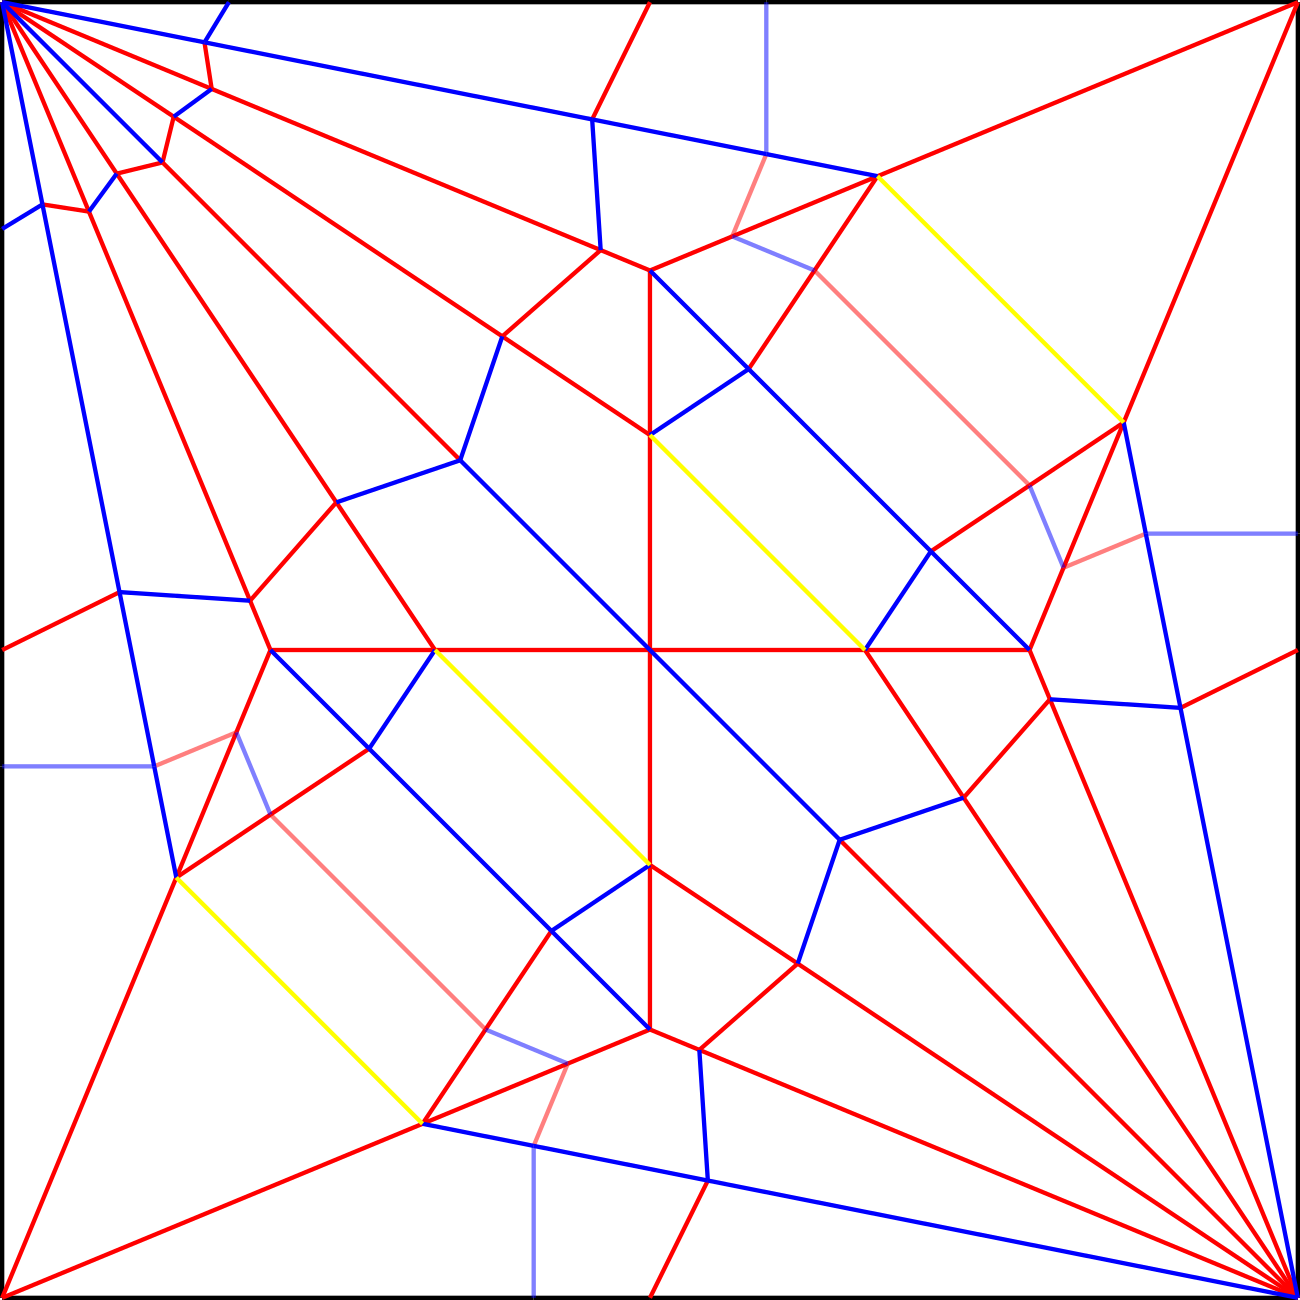
\includegraphics[width=0.8\textwidth]{assets/crane-crease-pattern.png}
\end{figure}

\subsection{Motivation}

Even though origami might seem to be a child's play, at times
people would get discouraged whilst following the origami instructions due to
the lack of details they expose.

We would like to provide a way, for beginners and advanced origamists alike,
to visualize the folding process step by step.
While there exist some programs aiding the process of design\cite{app:treemaker}\cite{app:omto}\cite{app:origami-draw}, there is no satisfactory solution 
that would present the process of folding the way it would be carried out manually.

We have evaluated existing products, and the one that resembles 
what we would like to achieve the most\cite{origami-simulator} provides a way to load a crease pattern
and view the folding process. 
However, it goes immediately from a flat sheet of paper to the folded figure, skipping all the steps
that would be required while folding the figure by hand.
It also bypasses some physical properties that we would like to achieve, such as the fact that the
paper should not interpenetrate itself.


\begin{figure}[H]
\caption{Origami simulator by Amanda Ghassaei}
  \centering
    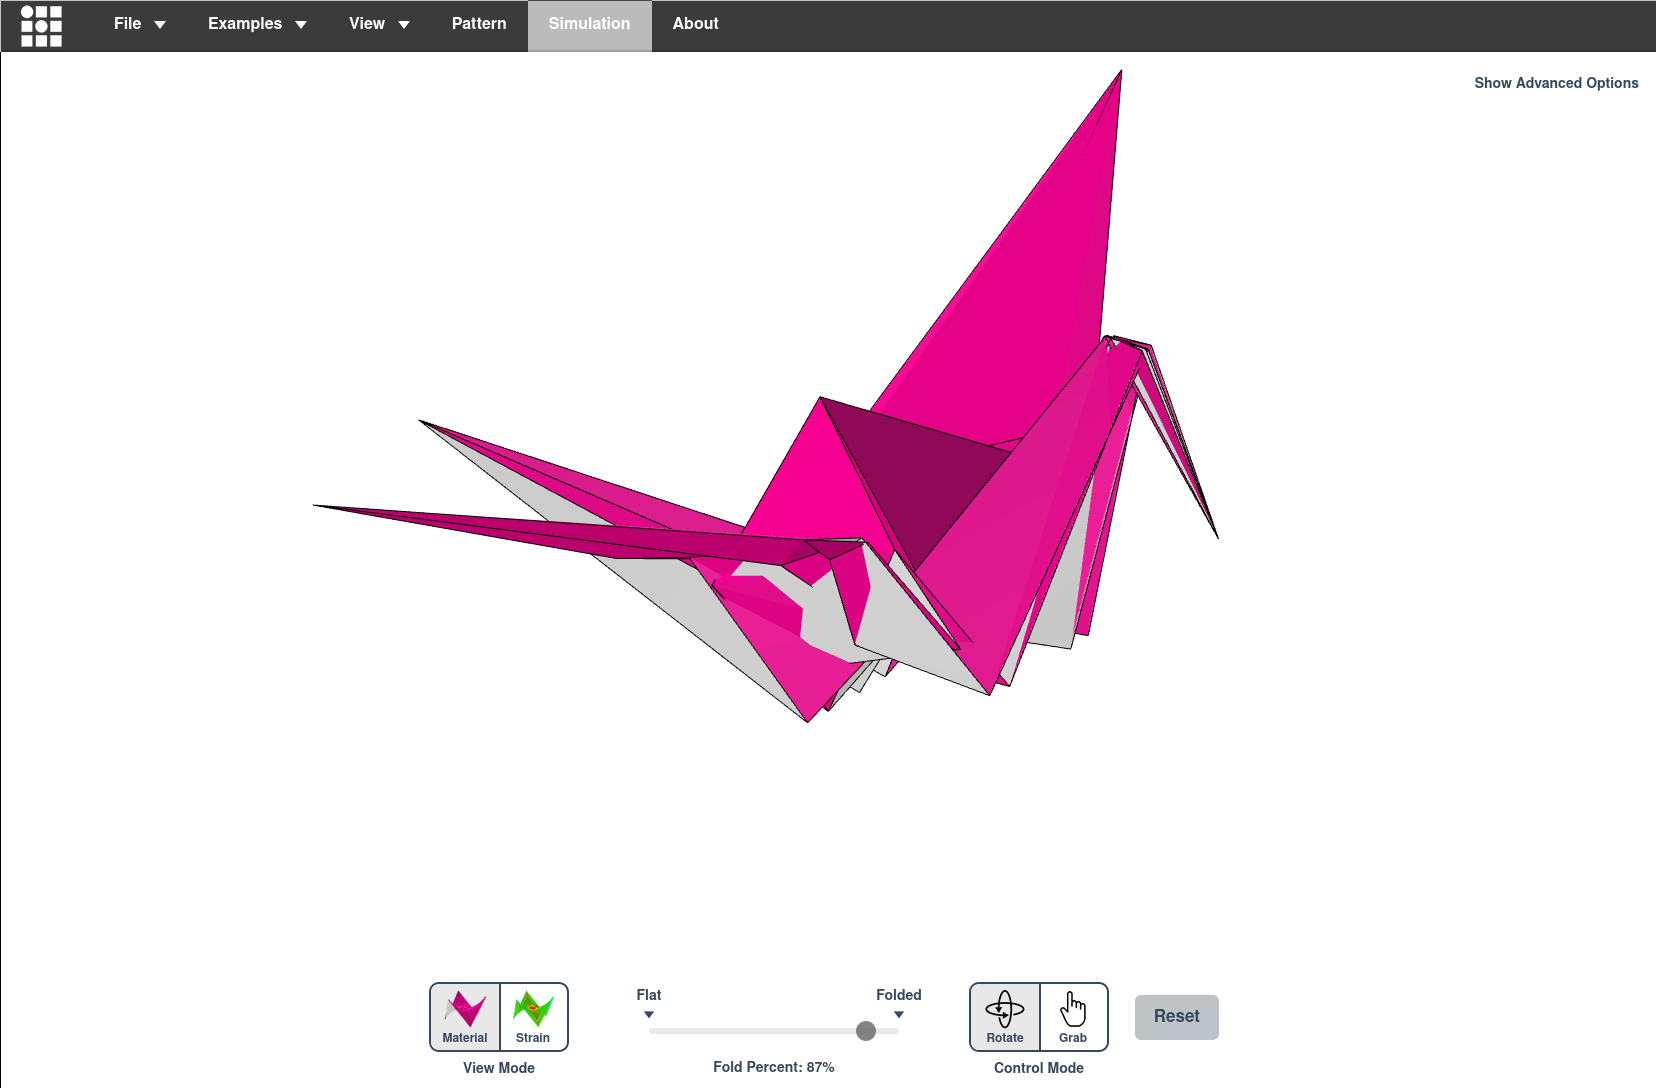
\includegraphics[width=\textwidth]{assets/origami-simulator.png}
\end{figure}

\clearpage 

\subsection{Product Vision}

\subsubsection{Functionality}

Our main goal is to create a platform that would allow visualisation of the origami folding process in a 3D space.
It would be possible to see how the figure folds at each step by playing an animation of the transition.

The inseparable component of the system would be a file format describing the folding sequence necessary to complete the origami figure.\\

The users in our system would at least be able to:
\begin{itemize}
	\item load a folding instruction,
	\item choose a step they want visualized,
	\item rotate the scene,
    \item zoom in and out,
	\item move around the scene,
	\item pause the animation at any time, and move back and forth.
\end{itemize}

\subsubsection{Technology}

Our application will consist of two layers -- backend and frontend.

The backend part will be responsible for storing user files and turning Instructions into animated Guides.
The frontend part will handle user interactions and 3D visualisations.

We have decided to use well-known and widely spread technologies.
For the backend part we will take advantage of \tech{Python} language with \tech{Django} framework.
As a data storage, we are going to incorporate \tech{PostgreSQL}.

For the frontend, we will use \tech{JavaScript} with \tech{React} for building the user interface.
The 3D rendering will be performed using \tech{Three.js} library that is built on top of \tech{WebGL} renderer.

\begin{figure}[H]
	\caption{Technology stack}
	\centering
	\begin{tikzpicture}
	\node (backend) at (0,0) [draw,thick,minimum width=4cm,label=north west:Backend] {
		
\includegraphics[width=.15\textwidth]{assets/python.png}
		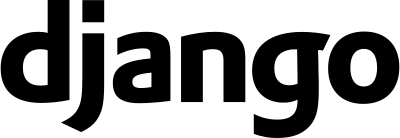
\includegraphics[width=.15\textwidth]{assets/django-logo.png}
	};
	\node[below = of backend] (frontend) [draw,thick,minimum width=4cm, label=north west:Frontend] {
		
\includegraphics[width=.12\textwidth]{assets/javascript-logo.png}
		
\includegraphics[width=.12\textwidth]{assets/react-logo.png}
		
\includegraphics[width=.23\textwidth]{assets/three-js-logo.png}
	};
	\draw[<->,thick] (backend.south) -- (frontend.north);
	\end{tikzpicture}
\end{figure}


\subsection{Feasibility Study}

Both \tech{Python} and \tech{JavaScript} are widely spread and actively maintained.
There is a strong community surrounding both of them.
\tech{Three.js} is the most popular library for 3D \tech{WebGL} rendering.

Therefore, we are not expecting problems connected with the tools we have selected.

Since the project will require a lot of knowledge from the \textit{computational origami}
field, we will have to research the existing materials on this topic.
The most promising resources seem to be the MIT course by
Eric Demaine\cite{mit-course} and a book co-authored by the same person -- \textit{Geometric Folding Algorithms: Linkages, Origami, Polyhedra}\cite{origami-book}.
Various available papers might come in handy as well, especially the ones regarding software implementations of origami folding algorithms.


\subsection{Threat Assessment}

Playing with the intersection between reality and computer science has always been a challenging task.
As the field of \textit{computational origami} is relatively young\cite{recent-results-in-computational-origami:paper}, there are still many obstacles to overcome.
As of now, the mathematical rules governing the origami folding are not fully developed.
On top of it, we are going to tackle a problem that has not been widely discussed.

Taking all of that into account, we foresee many challenges along the way, such as:

\begin{itemize}
	\item NP-hardness - some problems that we will face are proved to be NP-hard.
		Computing layer ordering based on a crease pattern is an example of such a problem.
		We will have to overcome them, either by using approximate methods or coming up with solutions that will avoid them.

	\item Physical properties of paper - should we support more complex physical properties,
		there are many features that would require a separate set of computations simulating paper physics, e.g.
		\begin{itemize}
			\item inflating,
			\item curving,
			\item cutting.
		\end{itemize}

	\item Performance -- web browsers are still not fully optimized to carry out 3D computations and render 3D graphics in real time.
		The system will have to be highly optimized in order to be usable.
		
	\item Mathematics -- we have little experience writing complex simulations utilizing complicated mathematical formulas.
		Even modelling a simple paper fold requires a lot of knowledge on different physical properties and frameworks that one could use.

	\item 3D graphics -- we have some experience working with 3D, however only from the user perspective.
		We have little experience in creating 3D graphical software.

\end{itemize}

Having said that, we believe we are capable of undertaking this problem and providing a solution to it.
Albeit challenging, it is rewarding especially in terms of projected business value and gained expertise.

\subsection{Dictionary}\label{dictionary}

\begin{description}
	\item[computational origami] \label{dictionary:computational-origami} -- a recent branch of computer science studying efficient algorithms for solving paper-folding problems.\cite{recent-results-in-computational-origami:paper}
	\item[crease] -- a line segment, along which a sheet of paper folds.
	\item[crease pattern] \label{dictionary:crease-pattern} -- a pattern of lines formed by creases that is created after unfolding the origami flat. For an example see figure \ref{fig:creasepattern}.
	\item[folded state] \label{dictionary:folded-state} -- An assembled origami model. Or alternatively, a sheet of paper folded along the crease pattern.
	\item[mountain] -- a fold of paper along the crease, such that the facets on the sides of the crease are facing downwards.
					\begin{figure}[H]
						\caption{Example of a mountain crease}
						\centering
						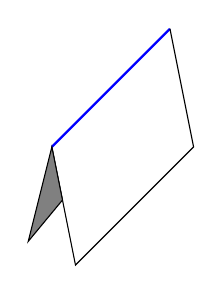
\begin{tikzpicture}[scale=1.5]
							\draw[blue, thick] (0,0) -- (1,1);
							\draw (1,1) -- (1.2, 0) --  (0.2, -1) -- (0,0);
							\filldraw[fill=gray] (0, 0) -- (-0.2, -0.8) -- (0.09, -0.45) -- cycle;
						\end{tikzpicture}
					\end{figure}
	\item[valley] -- A fold of paper along a crease, such that the facets on the sides of the crease are facing upwards.
					\begin{figure}[H]
						\caption{Example of a valley crease}
						\centering
						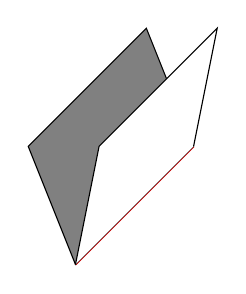
\begin{tikzpicture}[scale=1.5]
							\draw[red, thick] (0,0) -- (1,1);
							\filldraw[fill=gray] (0, 0) -- (-0.4, 1) -- (0.6, 2) -- (1, 1) -- cycle;
							\filldraw[fill=white] (1,1) -- (1.2, 2) --  (0.2, 1) -- (0,0);
						\end{tikzpicture}
					\end{figure}
	\item[mountain-valley assignment] -- an assignment of mountain or valley to the creases on the crease pattern.
	\item[.fold file] -- a file that conforms to the FOLD\cite{fold:paper} specification.
	\item[Instruction] -- a \textit{.fold} file created by a user, representing a sequence of steps required to
		fold a sheet of paper into a complete origami figure.
	\item[Transition] -- a folding animation played between two steps.
	\item[Guide] -- a set of all Transitions derived from an Instruction. Can be represented using a \textit{.fold} file.
	\item[Model] -- 3D representation of an origami figure. 
	\item[FPS] -- frames per second.
	\item[target angle] -- the supplement of the dihedral angle between the two neighbouring faces,
		towards which the faces should fold.
\end{description}




\clearpage

\section{\SectionTitleScope}
\label{sec:functionality}
\subsection{System actors}

Based on the requirements analysis, we have determined two types of actors in our system:

\begin{description}
	\item[Folder] \label{actors:folder} - A person who carries out the most important functionality in our system,
		that is - folds origami figures following the provided interactive instruction.
		This person does not need to have any special knowledge about origami creation nor the simulation process.
	\item[Designer] \label{actors:designer} - A person who is responsible for providing folding instructions
		for other users (\textit{folders}).
		A Designer is required to have basic knowledge about origami construction
		and interaction with the system to be able to create and upload an Instruction.
\end{description}

\newcommand{\requirement}[2]{\item #2. (#1)}
\subsection{Functional requirements}
\label{section:functional-requirements}

We define functional requirements for the system as User Stories grouped by actor type.
They have a priority assigned to them that ranges from 1 to 3. Where:

\begin{enumerate}
	\item[(3)] high priority - a feature required for the system functionality 
	\item[(2)] medium priority - a feature that is important, but not essential for the system functionality
	\item[(1)] low priority - a feature that is nice to have, but not required 
\end{enumerate}

\subsubsection{Folder user stories}
As a folder I am able to\ldots
\begin{enumerate}
	\requirement{3}{load an Instruction}
	\requirement{3}{view the 3D representation of the Instruction step}
	\requirement{3}{switch to the next step in the Instruction}
	\requirement{3}{switch to the previous step in the Instruction}
	\requirement{3}{see the Transition between two Instruction steps}
	\requirement{2}{pause the Transition at any time}
	\requirement{2}{rewind the Transition}
	\requirement{2}{forward the Transition}
	\requirement{3}{rotate the Model in 3D space}
	\requirement{3}{zoom the Model in and out in 3D space}
	\requirement{1}{see creases of the Model} 
	\requirement{2}{distinguish paper's top and bottom sides} 
	\requirement{1}{change the color of the paper side} 

	\requirement{3}{navigate between simulator and community views} 
	\requirement{3}{view Instructions uploaded by other users} 

	\requirement{3}{create an account} 
	\requirement{3}{log into the system} 
	\requirement{3}{reset the password} 
	\requirement{2}{change the password} 
	\requirement{2}{delete the account} 
	\requirement{2}{save another user's Instruction in my account} 
	\requirement{1}{mark a saved Instruction as folded} 
\end{enumerate}

\subsubsection{Designer user stories}
As a designer I am able to\ldots
\begin{enumerate}
	\requirement{3}{upload an Instruction}
	\requirement{3}{view my Instructions}
	\requirement{3}{delete my Instructions}
	\requirement{3}{update my Instructions}
	\requirement{1}{mark my Instructions as public or private}

	\requirement{1}{visually design an Instruction}
	\requirement{1}{save a designed Instruction}
\end{enumerate}

\subsection{Non-functional requirements}

We have deduced the following non-functional requirements that our system
needs to fulfill in order to meet the client's expectations.

\begin{enumerate}
	\requirement{3}{Anyone with an up to date web browser is able to use the application}
	\requirement{3}{The application must be reachable under a public address}
	\requirement{1}{All system components can be run on separate machines}
	\requirement{2}{Transitions should be played in at least 24 FPS on modern hardware}
	\requirement{1}{User should be able to use the application on mobile devices}
\end{enumerate}

\subsection{UI wireframes}

Based on the requirements, we have created the following UI wireframes that
present the most important parts of our system.


\begin{figure}[H]
\caption{Guide Viewer view}
  \centering
    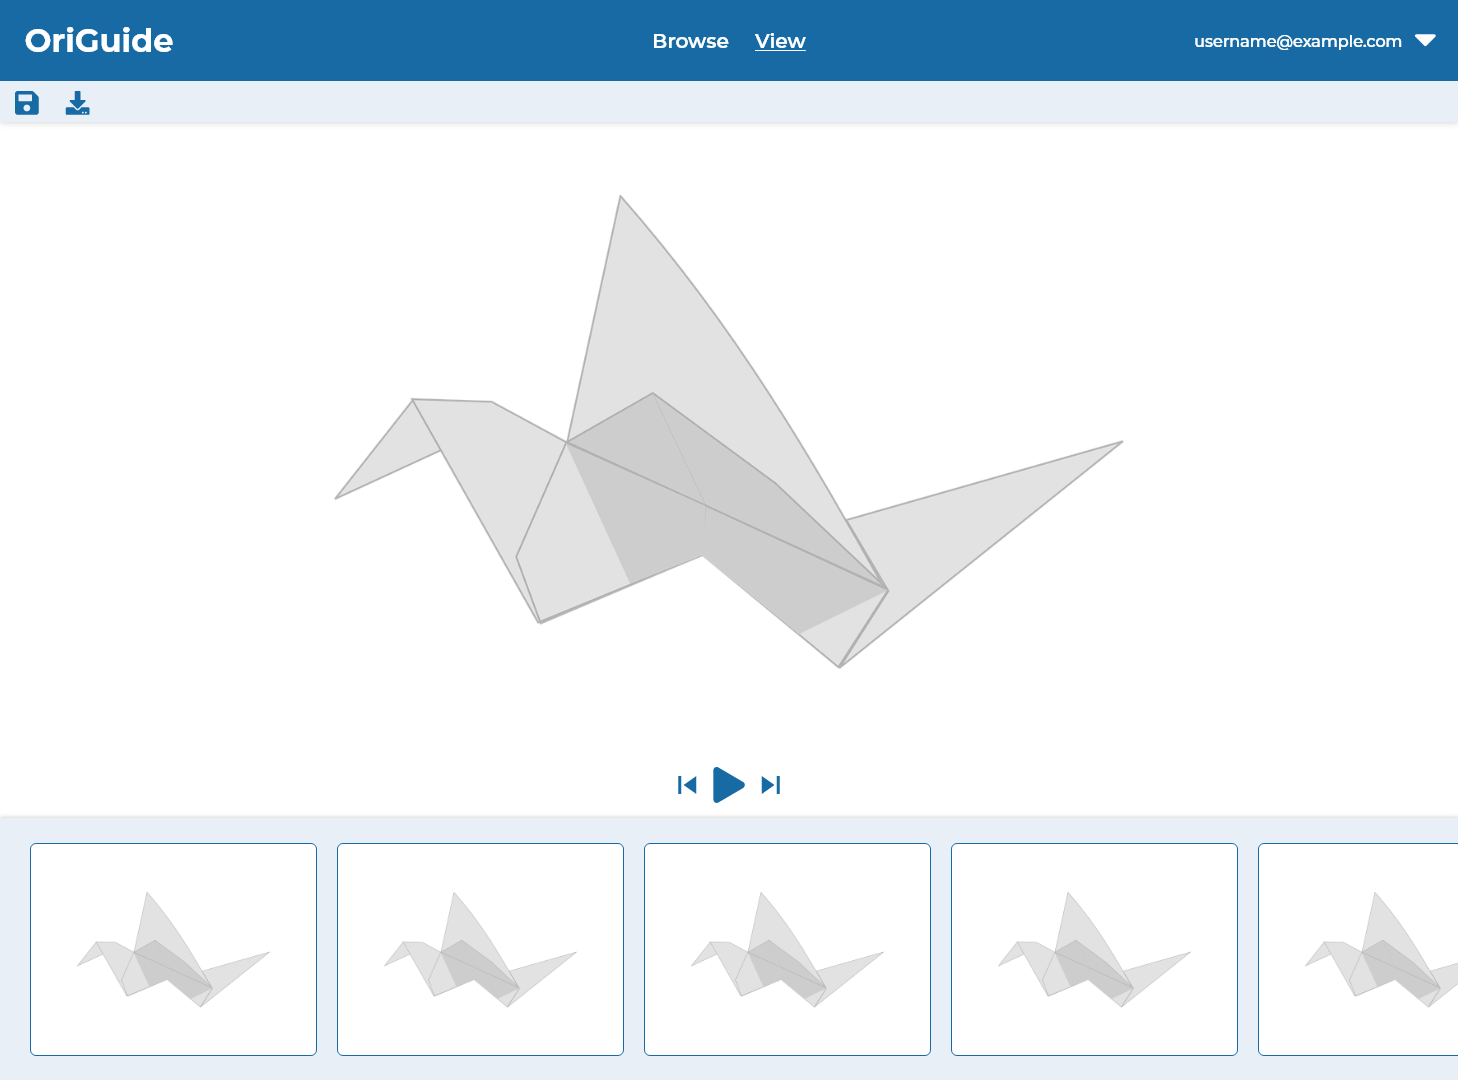
\includegraphics[width=0.8\textwidth]{assets/simulator-wireframe.png}
\end{figure}

\begin{figure}[H]
\caption{Community view}
  \centering
    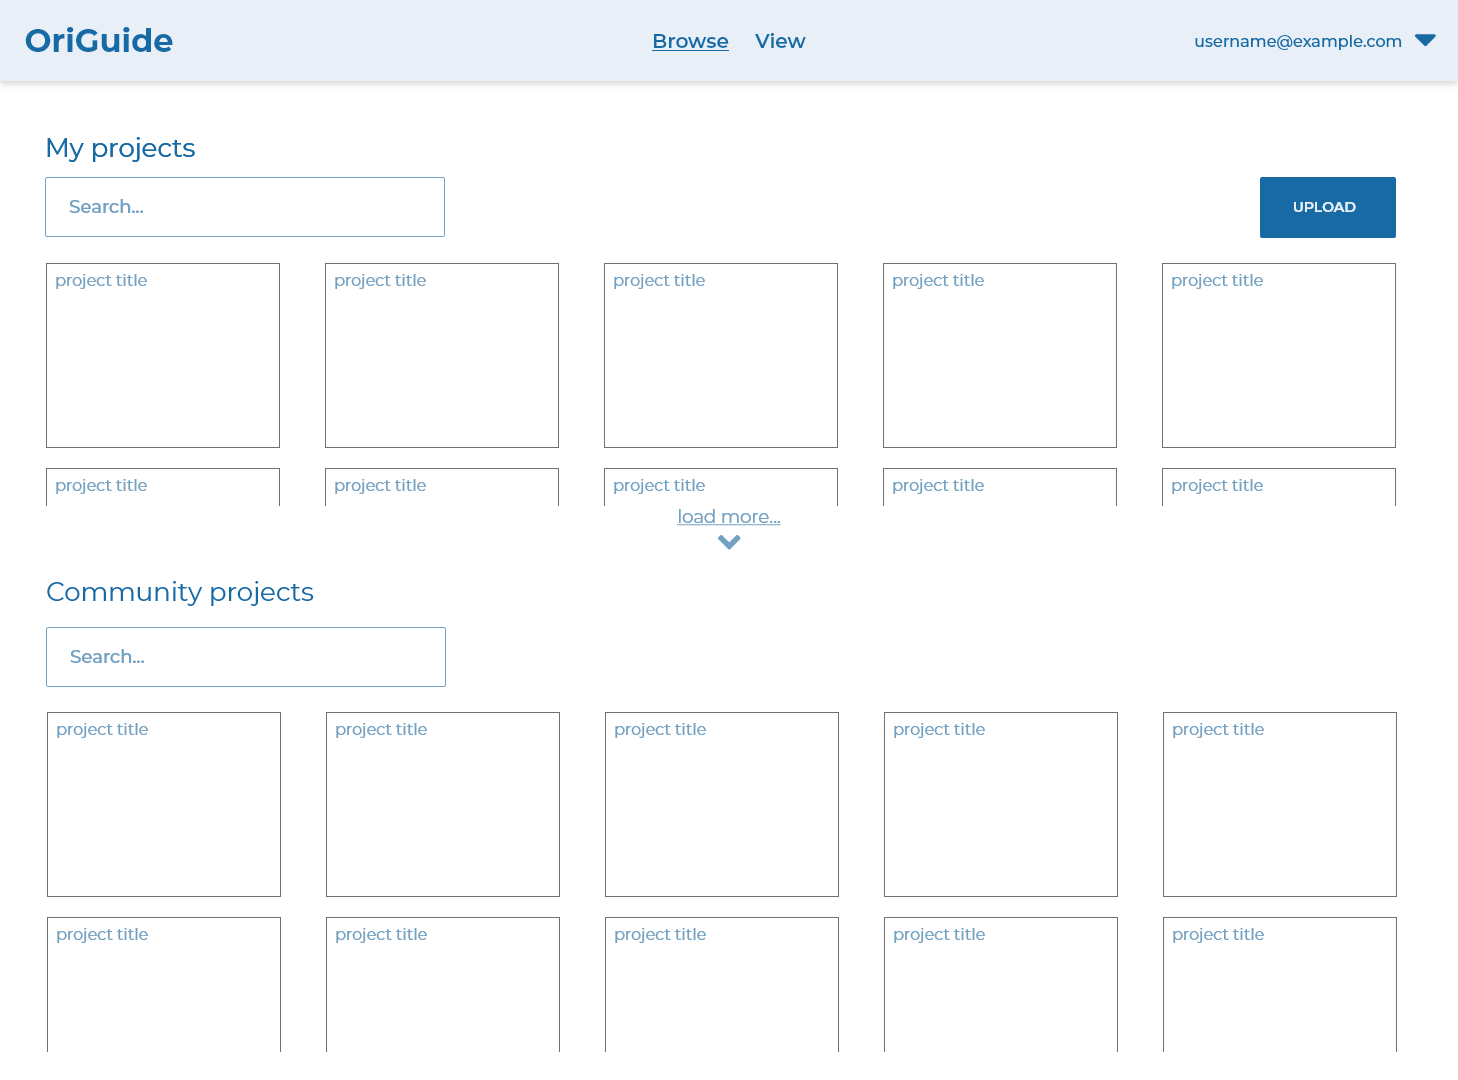
\includegraphics[width=0.8\textwidth]{assets/browser-wireframe.png}
\end{figure}


\section{\SectionTitleImplementationAspects}
\label{sec:implementation}
\subsection{Prototype}

From the list of features mentioned in the previous chapter we have selected the most important ones and created a prototype in a form of MVP (Minimum Viable Product). 

The selected features:

\begin{enumerate}
	\requirement{3}{load an Instruction}
	\requirement{3}{view the 3D representation of the Instruction step}
	\requirement{3}{switch to the next step in the Instruction}
	\requirement{3}{switch to the previous step in the Instruction}
	\requirement{3}{see the Transition between two Instruction steps}
	\requirement{2}{pause the Transition at any time}
	\requirement{2}{rewind the Transition}
	\requirement{2}{forward the Transition}
	\requirement{3}{rotate the Model in 3D space}
	\requirement{3}{zoom the Model in and out in 3D space}
	\requirement{1}{see creases of the Model} 
	\requirement{2}{distinguish paper's top and bottom sides} 
\end{enumerate}

Some of the listed functionalities require a numerical solver which is also included in the MVP.

Both Instructions and Transitions are represented using .fold files which we have extended with information required by the application.

\subsubsection{Frontend}

At first we had decided to use plain \tech{JavaScript} with the \tech{Rollup} bundler and \tech{Three.js} framework.
It quickly became apparent that the lack of state management will become problematic as the development progresses. Following that realization we have decided to incorporate a reactive framework - \tech{React} to aid the project with basic layout and aforementioned state manipulation. 
Due to minor interoperability issues the Rollup was also replaced with \tech{Webpack}.

The quality assurance is achieved through the use of:

\begin{description}
\item[Code linter] - EsLint
\item[Code prettiefier] - Prettier
\item[Test Runner] - Jest
\item[Continuous integration] - Github Actions
\end{description}

The implementation is continuously delivered to \tech{Netlify} via Github Actions.


\begin{figure}[H]
\caption{Origami simulation view}
  \centering
    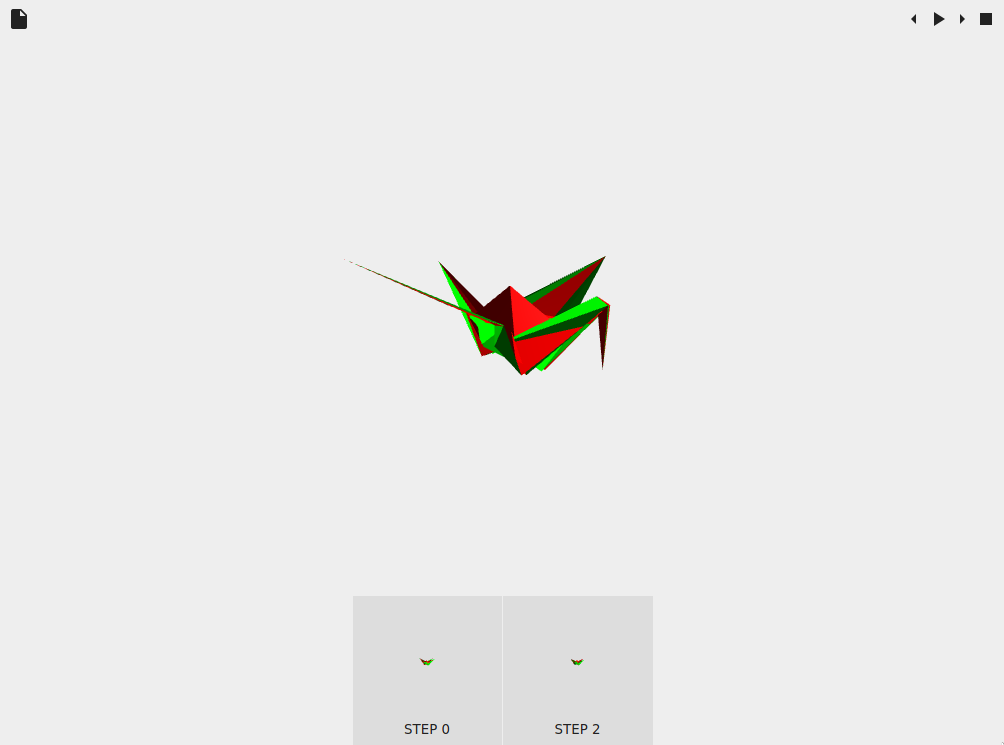
\includegraphics[width=0.8\textwidth]{assets/prototype-front.png}
\end{figure}

\subsubsection{Backend}

The current backend part is responsible for carrying out numerical computations.
It converts a provided Instruction into a set of coordinates representing
transitions between folding steps.\\

The solver is based on the techniques presented in the publication by A. Ghassaei.\cite{origami-simulator}.

The computational framework consists of the three most important forces,
that drive the folding process.

\begin{description}
	\item[Beam force] - responsible for preserving edge length
	\item[Face force] - responsible for preserving the original face shape
	\item[Crease force] - responsible for folding
\end{description}

Given the current vertices' positions, and the mountain-valley assignment,
the solver computes forces imposed on vertices, and calculates their next position
using the forward Euler integration.

An additional \textbf{damping force} is introduced to prevent solver from
high frequency oscilations, assuring numerical stability under most conditions.\\

The solver is implemented in \tech{python}, using \tech{numpy} and \tech{scipy} libraries. 


\begin{figure}[H]
	\caption{Visualization of vertices (dots), and forces applied to them (arrows)
	during folding of a rectangular sheet of paper in half, along the diagonal. }
  \centering
    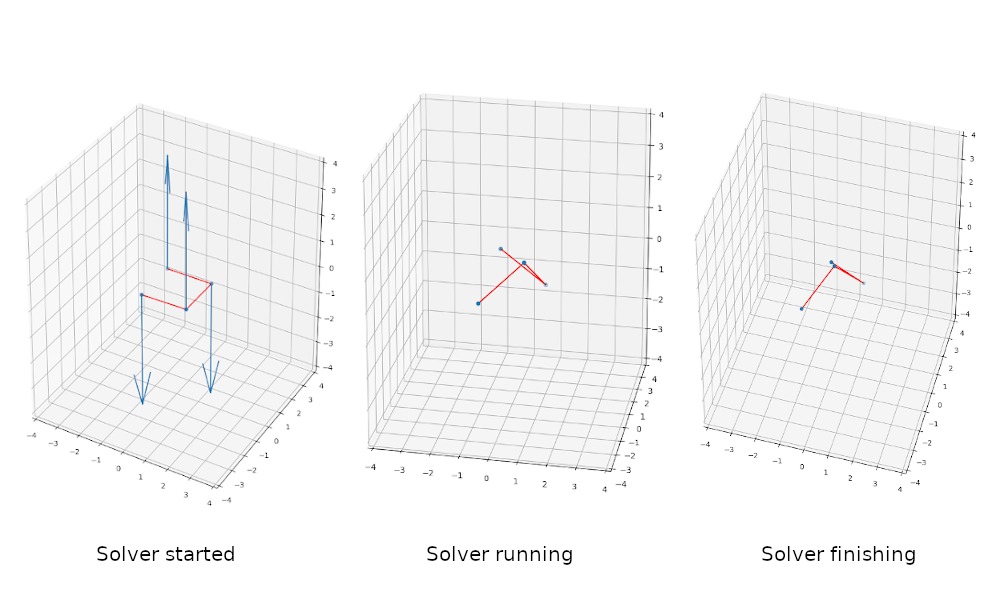
\includegraphics[width=0.8\textwidth]{assets/prototype-backend.png}
\end{figure}


\subsection{Project overview}

\begin{figure}[H]
	\caption{High level system overview}
  \centering
    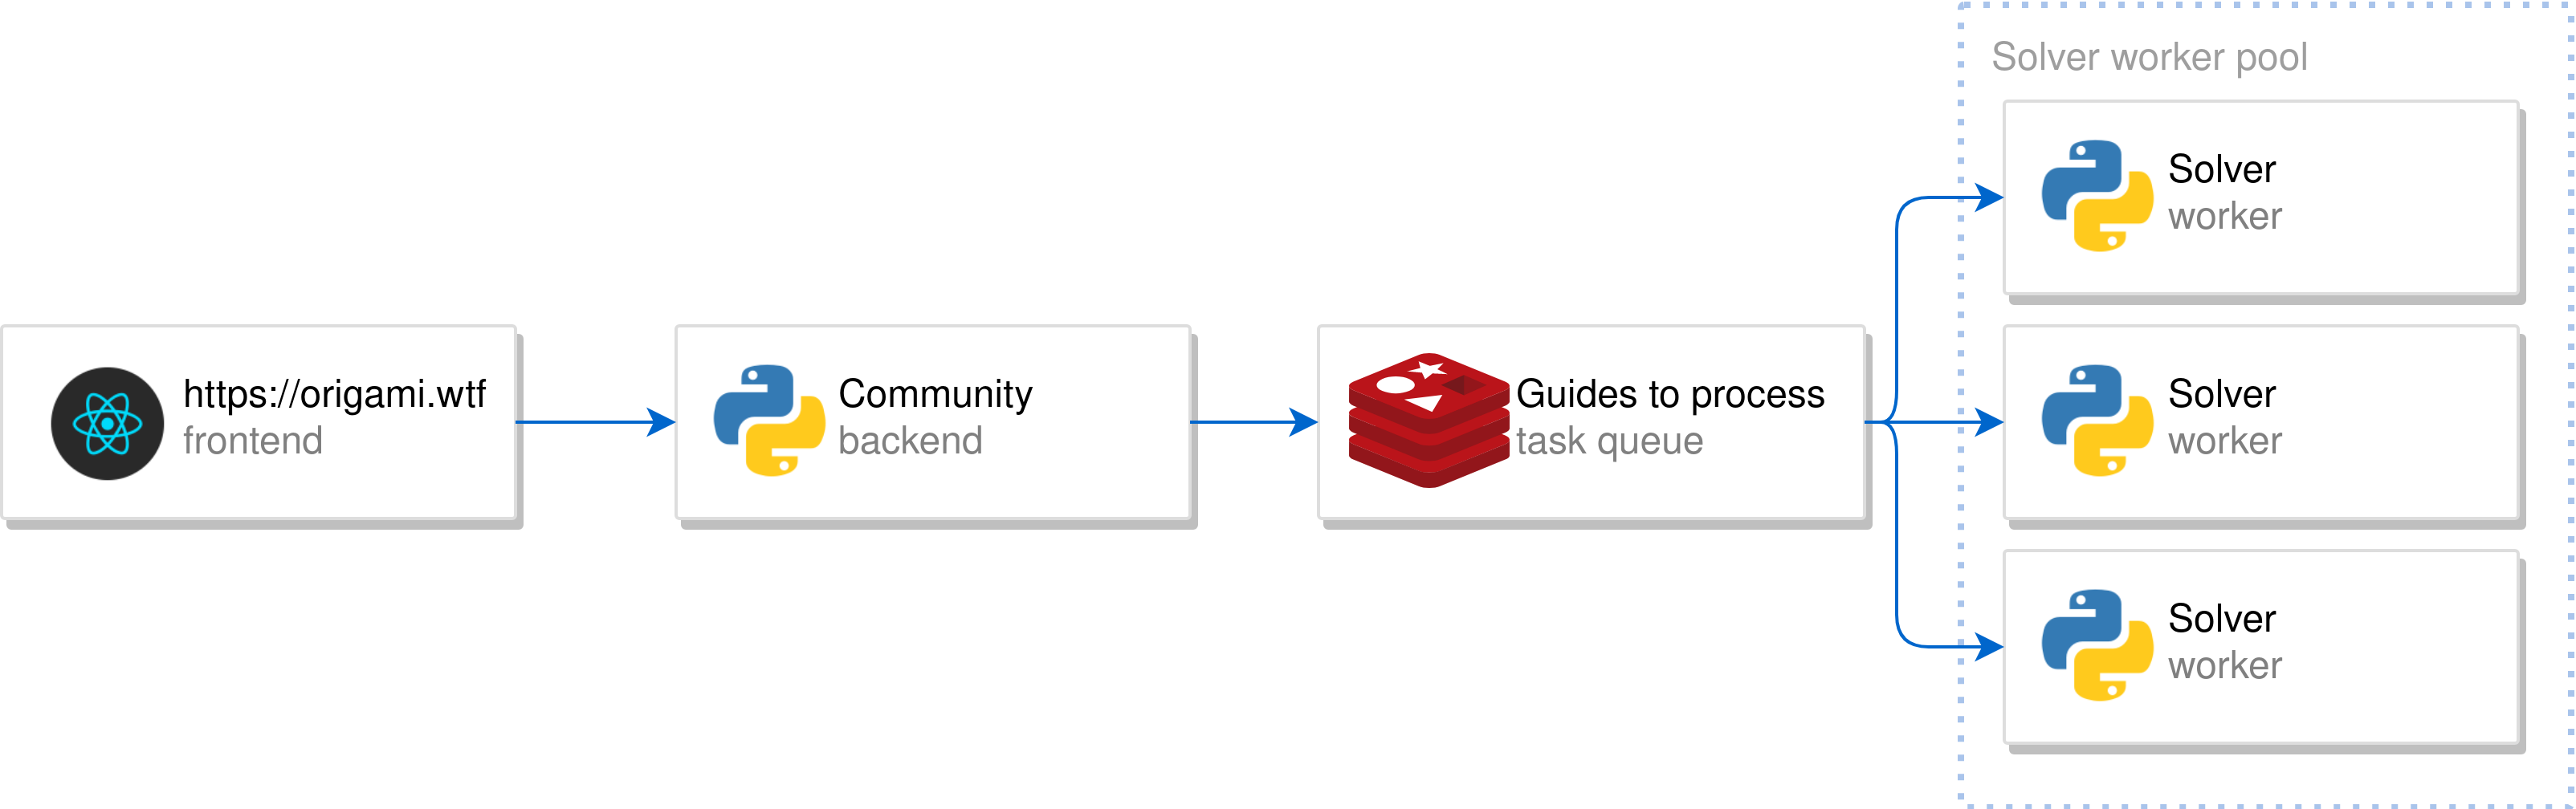
\includegraphics[width=\textwidth]{assets/architecture.png}
\end{figure}

Origuide consists of the following layers:
\begin{description}
	\item[Frontend] - a component that handles all user interactions with the system. 
	\item[Backend] - a component responsible for: \begin{itemize}
		\item processing all user requests initiated on the Frontend
		\item managing persistent data 
		\item authentication and authorization
		\item scheduling Guide processing
	\end{itemize}
	\item[Guides to process] - a task queue distributing guides to process among Solver workers
	\item[Solver worker] - a component responsible for converting Instructions to Guides.
\end{description}

As we previously distinguished two types of users in the system, there are two main success paths through the application.

\begin{figure}[H]
	\caption{Designer's success path}
  \centering
    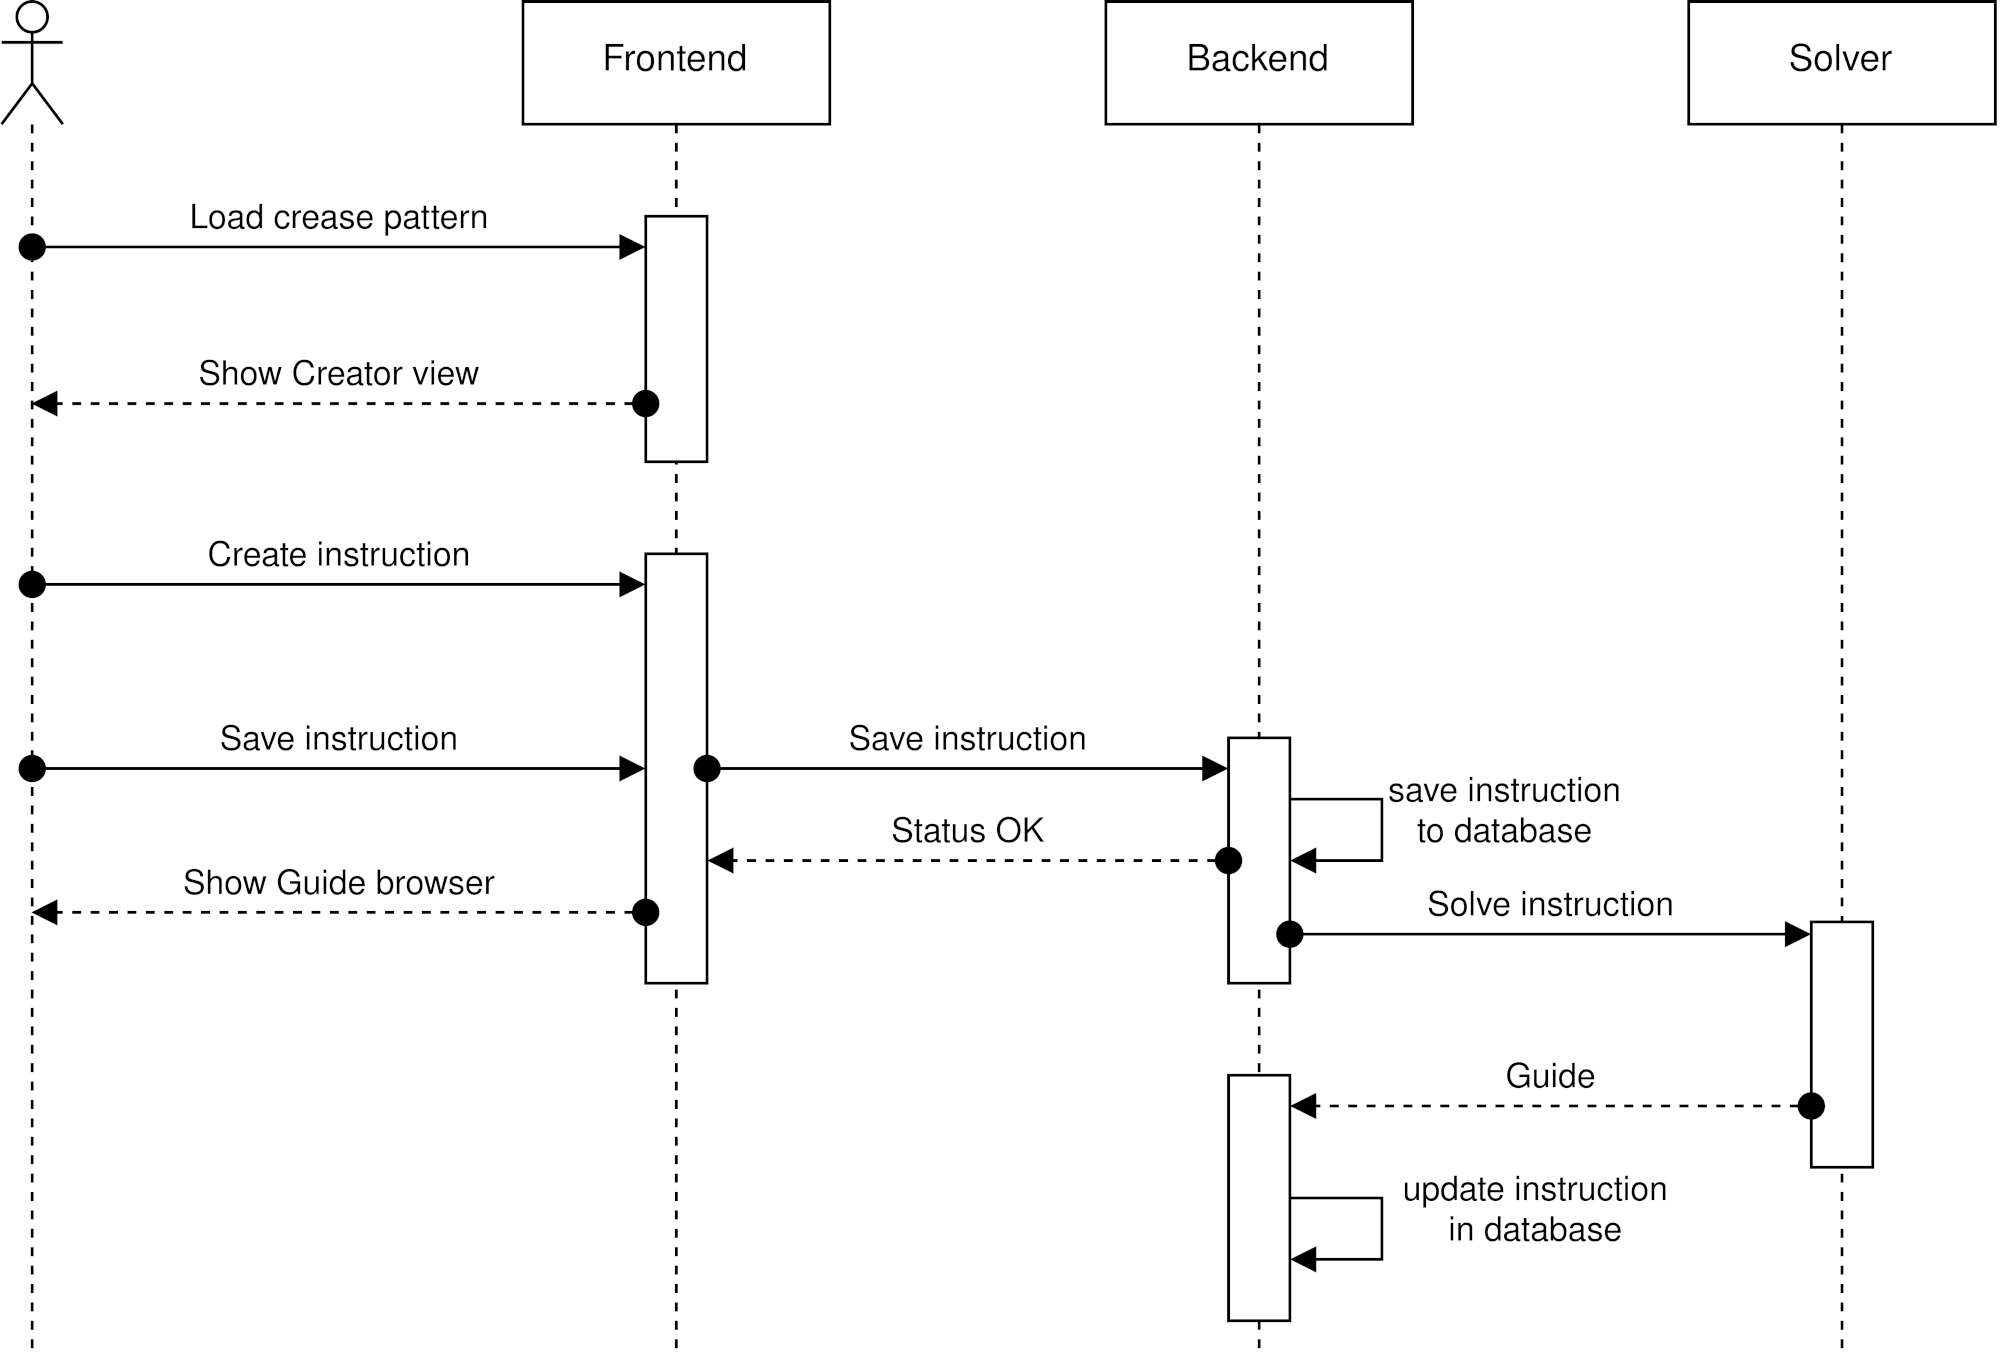
\includegraphics[width=\textwidth]{assets/3-designer-flow.png}
\end{figure}

Designer's main objective is to create Guides. After uploading a Crease Pattern, Designer is required to provide instruction steps. When an Instruction is saved it gets scheduled on a Task Queue and processed by a Solver worker. Once processing is finished the Instruction associatied with the Guide is marked as solved in the database.

\begin{figure}[H]
	\caption{Folder's success path}
  \centering
    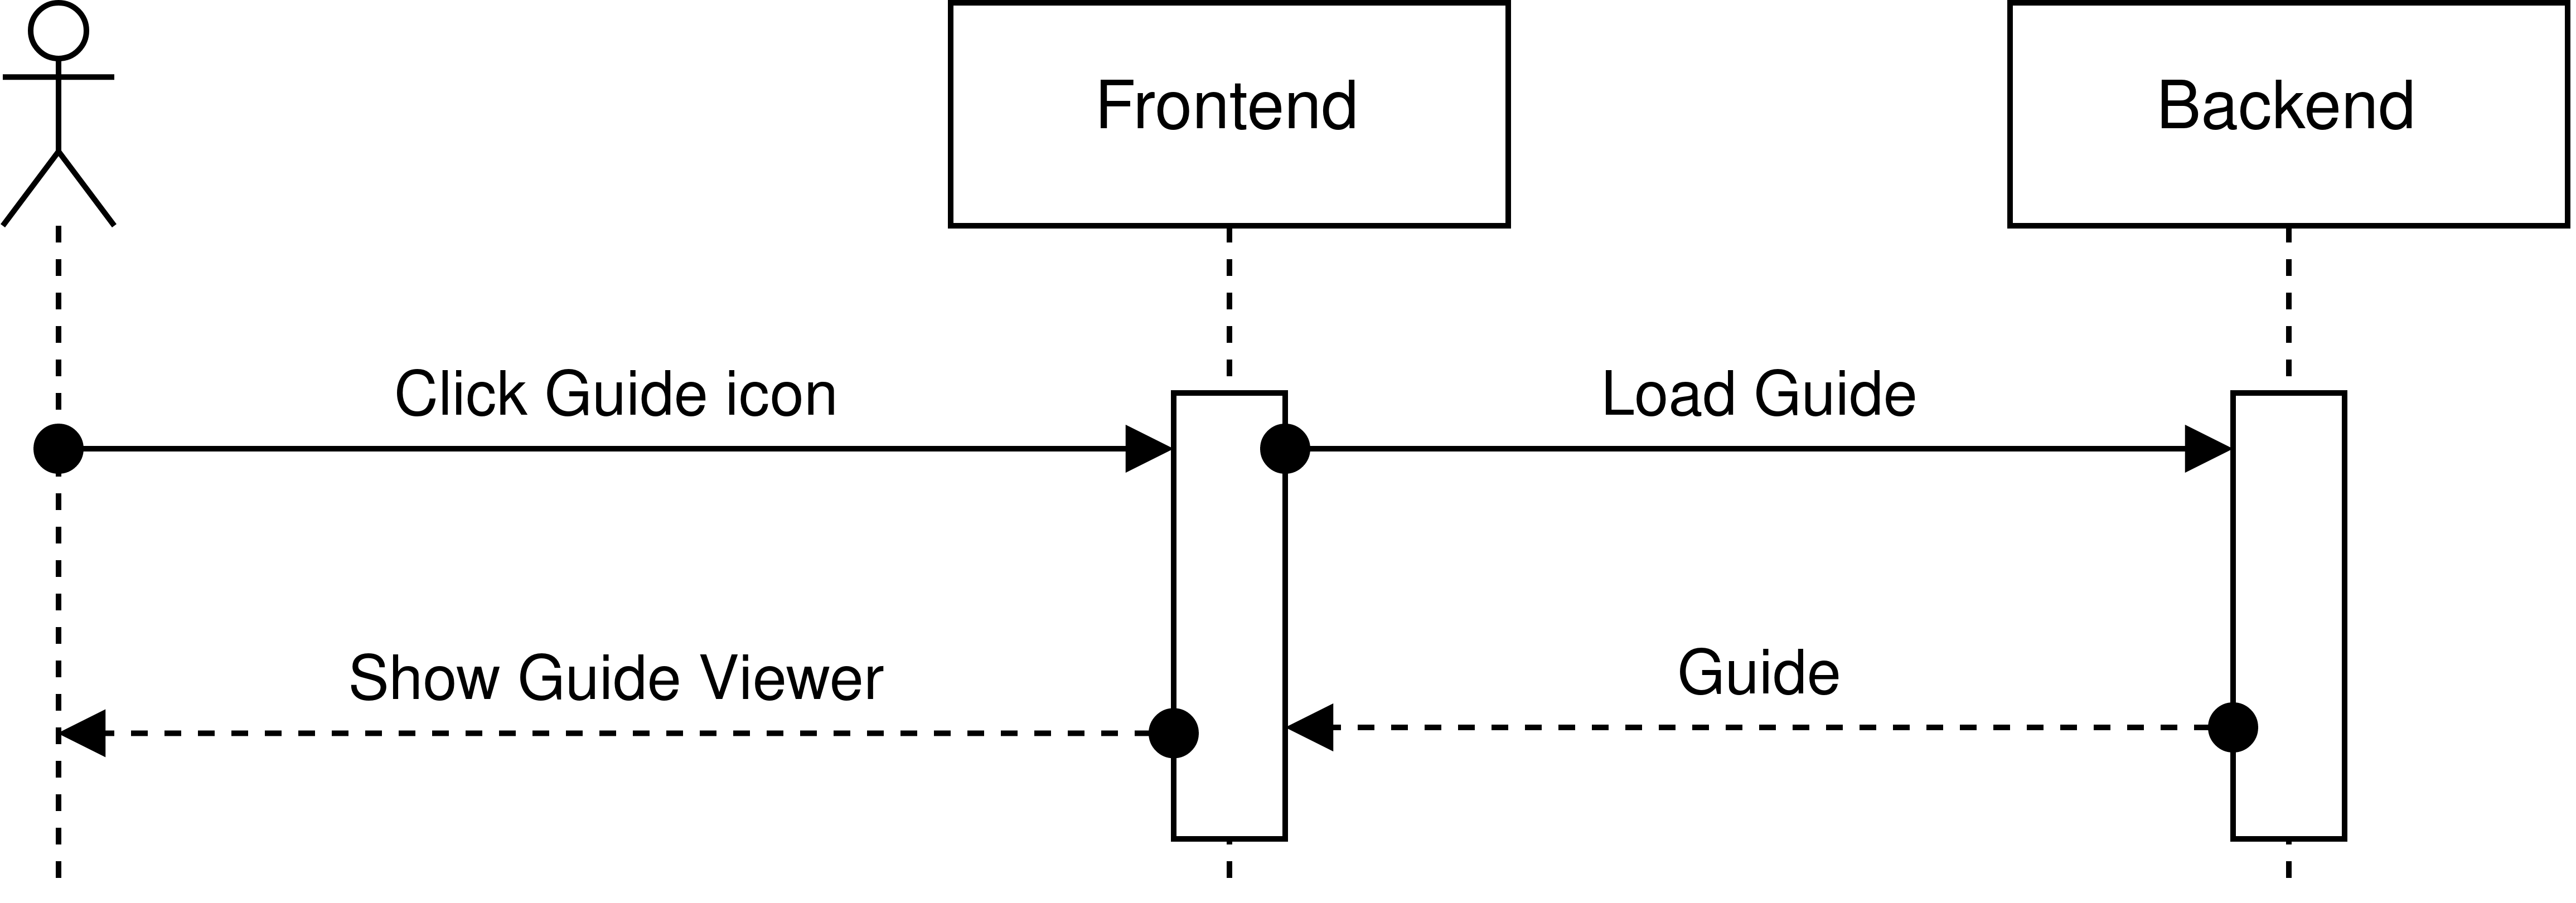
\includegraphics[width=\textwidth]{assets/3-folder-flow.png}
\end{figure}

Folder's main objective is to fold origami figures following steps presented by the Application. After successfully retrieving a guide from the Backend, he is presented with a Guide Viewer.

\subsection{Technology stack}

Source Code is version controlled using a hosted \tech{Git} solution - \tech{Github}.  

Continuous Integration and Continuous Deployment is provided by \tech{Github Actions}. 

\subsubsection{Frontend}

\begin{itemize}
	\item The Application is built in \tech{Javascript} using \tech{React} framework. 
	\item \tech{Three.JS} is used to display 3D models.
	\item Triangulation is done using \tech{earcut}. 
	\item Parsing folds is aided by \tech{fold}.
	\item User Interface components come mainly from \tech{material-ui}.
	\item \tech{Webpack} is responsible for bundling, minimizing and transpiling the source code.
	\item Code style is checked using \tech{Prettier} with \tech{eslint} and enforced on every commit using \tech{Husky}.
	\item \tech{Jest} has been incorporated as a test runner.
\end{itemize}

// TODO: comment

\subsubsection{Backend}

\begin{itemize}
	\item The Backend is built in \tech{Python} using \tech{Django} framework. 
	\item \tech{DjangoRestFramework} simplifies a REST server setup.
	\item \tech{drf-base64} helps with decoding of base64 encoded files.
	\item \tech{PyJWT} assists in auth process.
	\item \tech{factory-boy} is used to generate testing data.
	\item Data is stored in a \tech{PostgreSQL} database.
	\item \tech{Celery} was chosen for an asynchronous task processing.
	\item \tech{Redis} acts as a task queue for \tech{Celery}.
\end{itemize}


\subsubsection{Solver}

\begin{itemize}
	\item Solver runs under \tech{Python}'s alternative implementation - \tech{PyPy}.
	\item \tech{Shapely} is used for triangulation.
\end{itemize}



\subsection{Components overview}
% Przegląd poszczególnych komponentów a wiec np. baza danych, aplikacja typu klient, serwis RESTowy. Jeśli baza to ERD z opisem, jeśli aplikacja kliencka to jakie elementy, widoki, jak się łączy i kiedy. Jeśli prosta aplikacja WWW to można pokazać strukturę projektu. Jeśli serwis RESTowy to jego specyfikacja z przykładami. Protokół komunikacji to może być zupełnie osobny opis. %

\subsection{Algorithms}
% Ciekawsze algorytmy, aspekty, mechanizmy np. logowanie, indeksowane, cachowanie, synchronizacja, backup, jakieś procesy w tle, jakieś progress bary, jakieś analizy, generowanie warstw GISowych, lokalizacja etc. Jest tu często o czym pisać. %

\subsection{Development environment setup}
% Instrukcja postawienia środowiska deweloperskiego - jeśli potrzeba wypełniacza %

\subsection{Deployment}
% Instrukcja postawienia środowiska deweloperskiego - jeśli potrzeba wypełniacza %

\subsection{Quality assurance}
% Quality Assurance: czy mamy testy jednostkowe? Czy mamy inne testy automatyczne? Jakich bibliotek używacie? %
At every commit that is a part of the master branch or a Pull Request Unit Tests are run. \\

\subsection{Problems encountered}
% Z jakimi problemami technicznymi sie borykaliście? Jeśli nie opisaliście ich w dokumentacji procesowej. %


\clearpage

\section{\SectionTitleWorkOrganization}
\label{sec:organizacja-pracy}
\subsection{Project characteristics}
% Charakterystyka projektu i sposób jego realizacji - macie tutaj napisać co to był za projekt (badawczy, rozwojowy) a wiec czy wymagania były jasne czy tak naprawdę powstawały w jego trakcie. Ważne by spróbować scharakteryzować przyjęty sposób realizacji a wiec przyjęty proces np. czy to był proces przyrostowy czy iteracyjny. Najczęściej Wasz proces jest oparty na prototypowaniu z odrzucaniem przez pierwszy semestr, a potem to typowy proces przyrostowo-iteracyjny w drugim semestrze. Spróbujcie napisać również z czego to wynika.

Our projects is special for a few reasons.

First of all, we came up with a project idea ourselves and tried to find a person that would be interested in being a thesis supervisor.
Taking that into account, the requirements for the project were not defined beforehand
and we learned more and more about them as the project developed.
Due to that fact, it was both easier and harder for us to do our job as architects and developers.
On the one hand, it was mostly us who were responsible for the direction the project would take, but at the same time, at each step of the process
we had to struggle with choosing which parts of the project would be more attractive for our client, our future users, and from the scientific point of view.

Second of all, some of the problems we were faced with come from the field of \textit{Computational Origami}.
It's a relatively new branch of science, which ideas span the realms of mathematics, physics, 
computer science, engineering, and even architecture.
Also, it is not a subject that would normally be taught during one's educational career.
Of much help to us was Prof. Erik Demaine and his MIT course on Geometric Folding Algorithms: Linkages, Origami, Polyhedra \cite{mit-course}
\smallskip

Taking into consideration all the facts mentioned above, our work did not have a specifically structured approach.
We were working in a very simplified \textbf{Kanban} method, where we would select things to work on
as the project unfolded. 
\smallskip

For the better part of the first semester,
we were creating a prototype that would serve as a \textit{Minimal Valuable Product}.
Later on, we did not discard it altogether, but started adding more features on top of it,
polishing it and refactoring when necessary. 
We continued with this approach till the end.

\subsection{Team}
% Osoby w projekcie - często projekt jest robiony dla kogoś a opiekun ma jakieś osoby pomocnicze. Wskażcie wszystkie osoby i ich role w projekcie. Bardzo ważny punkt z formalnego widzenia projektu, gdyż każda osoba musi zostać oceniona w sposób indywidualny.

Our team consisted of our thesis supervisor and us.

\begin{enumerate}
	\item \textbf{Witold Alda} - thesis supervisor.
	\item \textbf{Maciej Mionskowski} - developer, architect.
	\item \textbf{Antoni Mleczko} - developer, architect.
\end{enumerate}

\subsection{Responsibilities in the team}
% Zespól i podział obowiązków - musicie napisać co kto robił. Jeśli wszystko robiliście razem to spróbujcie wskazać chociaż 2-3 główne zadania, którymi każde z Was się zajmowało.

Although we were distributing workload equally between the team members
and each of us touched on all parts of the project, some areas 
received more attention from one person than the other.
To be able to define how much of a percentage each one of us has contributed to the 
given area of the project, first we need to define those areas.
\smallskip

Project areas:
\begin{itemize}
	\item Solver backend
	\item Frontend
	\item Community backend
	\item DevOps / Infrastructure
	\item Thesis
	\item Research
	\item Requirements formulation
\end{itemize}

Having defined project areas, we have agreed upon how much of a contribution each of
us has provided to the given area.

\begin{figure}[H]
  \caption{Maciej's percentage contribution to the areas of the project.}
  \centering
  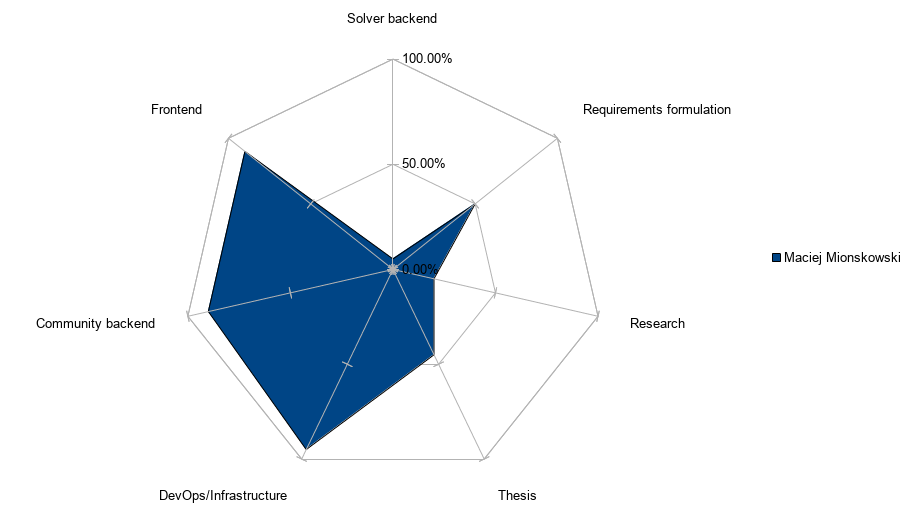
\includegraphics[width=\textwidth]{assets/4-percentage-maciej.png}
\end{figure}

\begin{figure}[H]
  \caption{Antoni's percentage contribution to the areas of the project.}
  \centering
  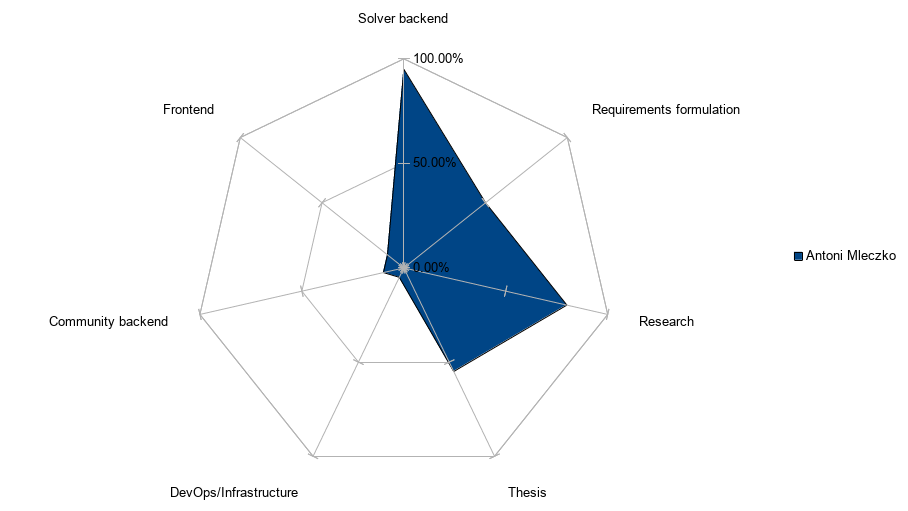
\includegraphics[width=\textwidth]{assets/4-percentage-antoni.png}
\end{figure}




\subsection{Organization of work}
% Organizacja prac i wykorzystane narzędzia - używaliście facebooka, emaili czy spotykaliście się zawsze o określonej porze? Jak i kiedy dzieliliście się zadaniami: czy było to po każdym spotkaniu z klientem? Kiedy spotykaliście się z klientem? Jak często? Używaliście Jiry, confluence, trello? Koniecznie zróbcie screenshota! A może jakieś statystyki z githuba które jakoś podsumują Wasz projekt? Tutaj Wasze przemyślenia i komentarze mile widziane.
% Zastosowane techniki i praktyki - odnosi się do powyższego, ale możecie tutaj spróbować wskazać takie praktyki jak Pair Programming, TDD, Refactoring, Planning Game, User Stories, Team Velocity, Continuous Integration, Sprint Review Meeting, makiety GUI. Jak wyglądał proces testowania? Czy były robione jakieś prototypy? Jak były walidowane, odrzucane (te kwestie ew. do dokumentacji technicznej)?

\subsubsection{Tools}

\tech{Github} was our provider of choice for hosting the code repository, planning work, incorporating continuous integration, continuous delivery, and tracking progress. Despite some of the project management  and CI related features on Github being relatively new and simple, they were suitable enough for our needs. Using the same service for managing all project aspects allows for natural cross-referencing between issues and code. It also acts as a single source of truth, hence reducing the hassle associated with jumping between platforms and keeping them synchronized. 

For creating diagrams we used \tech{diagrams.net} (formerly draw.io), \tech{canva.com}, and \tech{TikZ}. \tech{GIMP} was used for editing screenshots and graphics. System mock-ups were designed in \tech{Adobe XD}.

\subsubsection{Work methodology}

Our work methodology was simple, agile, and based on the Kanban system.

\medskip
We used multiple Github project boards to incorporate Kanban into our environment. 
Community Backend, Solver Backend, Thesis, and Infrastructure each received their separate Kanban Boards. Every Board could represent a separate team working on the project.

\begin{figure}[H]
  \caption{One of the many Kanban Boards in our project.}
  \centering
  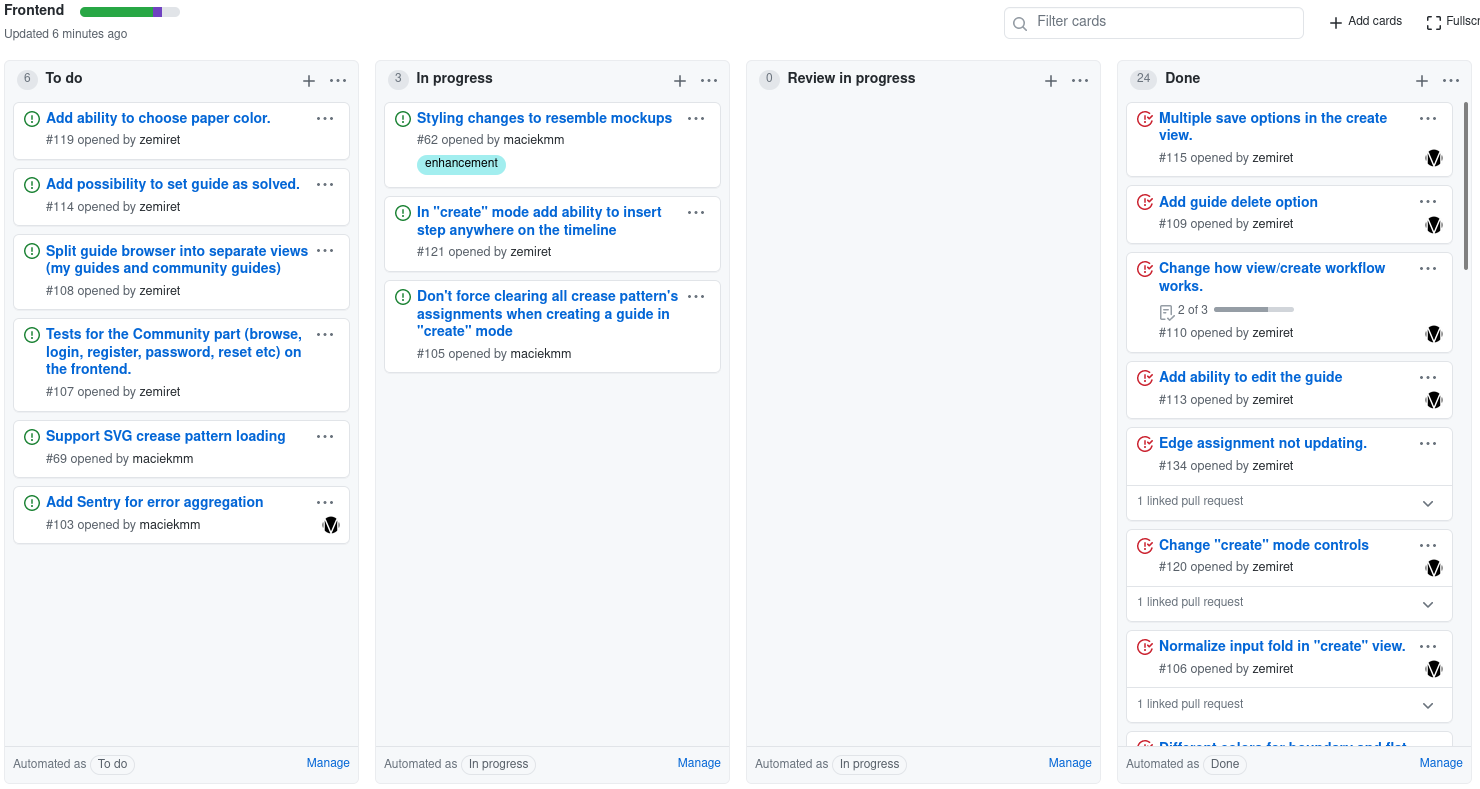
\includegraphics[width=\textwidth]{assets/4-gh-board.png}
\end{figure}

We would pick issues to work on by moving a card from the \textbf{To Do} to the \textbf{In progress} column. Once the development was finished and ready for a review, a Pull Request would be created and the card would be marked as \textbf{Review in progress}. Should a feature pass the review process, the card would be moved to the \textbf{Done} lane.

\medskip 

After we established all functional requirements, they acted as our guide for creating issues. Feature's priority impacted the position of the card in the \textbf{To Do} column. The more important the feature was, the higher it appeared on the \textbf{To Do} pane.

\subsubsection{Communication}

\textbf{Internal}

Thanks to all development team members working from the same place, most of the communication was carried out face to face. This fact had a positive impact on the project as ideas were communicated clearly and quickly. Non-urgent matters were handled through Github issues.

\medskip

\textbf{External}

E-mail was used as the main mean of information exchange between the developer team and the thesis supervisor. Occasionally, phone calls and \tech{Microsoft Teams} were used when a longer discussion was needed. The communication was established primarily in situations when we wanted to confirm a path the project is heading.


\subsubsection{Code development}

As a version control framework we used a simplified \tech{Git workflow}. Each feature would be first developed on a feature branch. Once the work was finished, a Pull Request would be created. The Pipeline would run tests against the changed components. Should the pipeline pass, the review process would commence. Once the work was successfully reviewed, the \texttt{master} branch would be rebased onto the feature branch to avoid merge conflicts. The Pull Request would then be squashed and merged into the \texttt{master} branch. The main branch would run the Pipeline with an additional delivery step, which would result in the code being published to the production environment.




\subsection{Project timeline}
% Przebieg prac (harmonogram, kalendarz): podział na poszczególne etapy, iteracje i jak one wyglądały i co było ich efektem.

The idea for the project was born in Februrary 2020, during a brainstorming session.
The project began in March 2020 and was finalized in December 2020.

\medskip

The general overview of the project timeline can be presented in four phases:
\begin{enumerate}
	\item \textbf{Brainstorming}, during which we held a couple of brainstorming sessions and came up with a few dozen of project ideas.
	\item \textbf{Idea Formalization}, in the midst of which we looked for a supervisor.
	\item \textbf{Topic Research}, throughout which we gathered required scientific knowledge.
	\item \textbf{Development}, during which we developed an actual product.
\end{enumerate}

The diagram below depicts the estimated phase lengths during the project time frame.

\begin{figure}[H]
\label{4-project-phases}
  \caption{Project phases timeline}
  \centering
    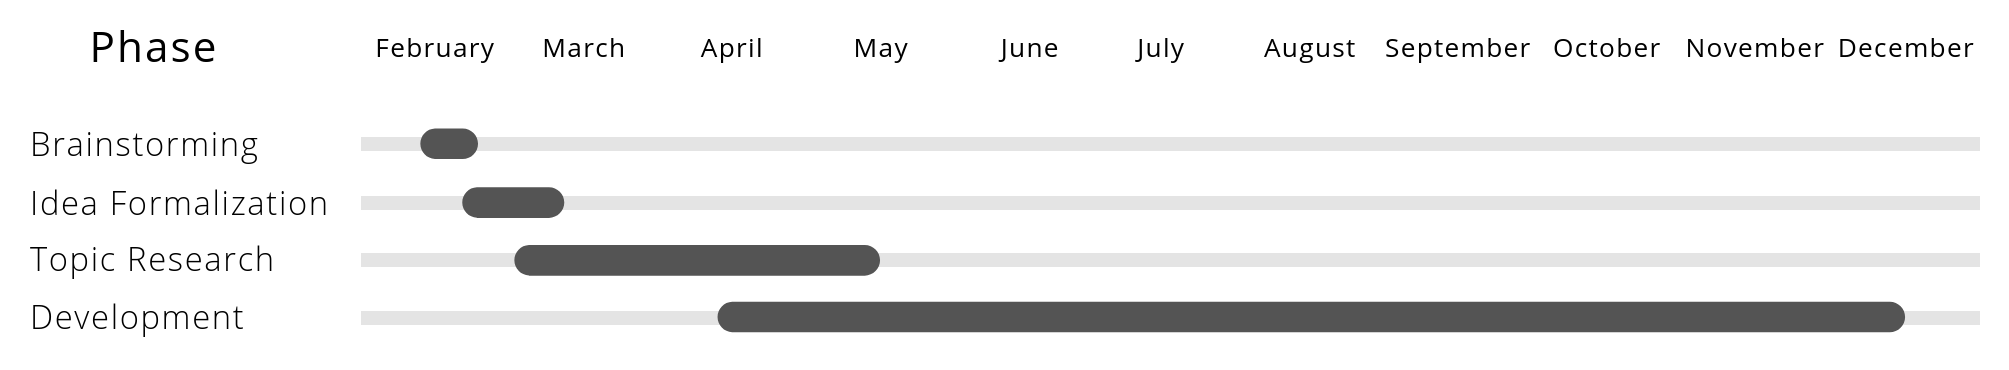
\includegraphics[width=\textwidth]{assets/4-phases.png}
\end{figure}

To see how different aspects of the project unfolded, a more detailed graphic has been created. The data has been mostly sourced from the project's code repository.

\begin{figure}[H]
	\label{04-component-timeline}
	\caption{Components development timeline}
  	\centering
    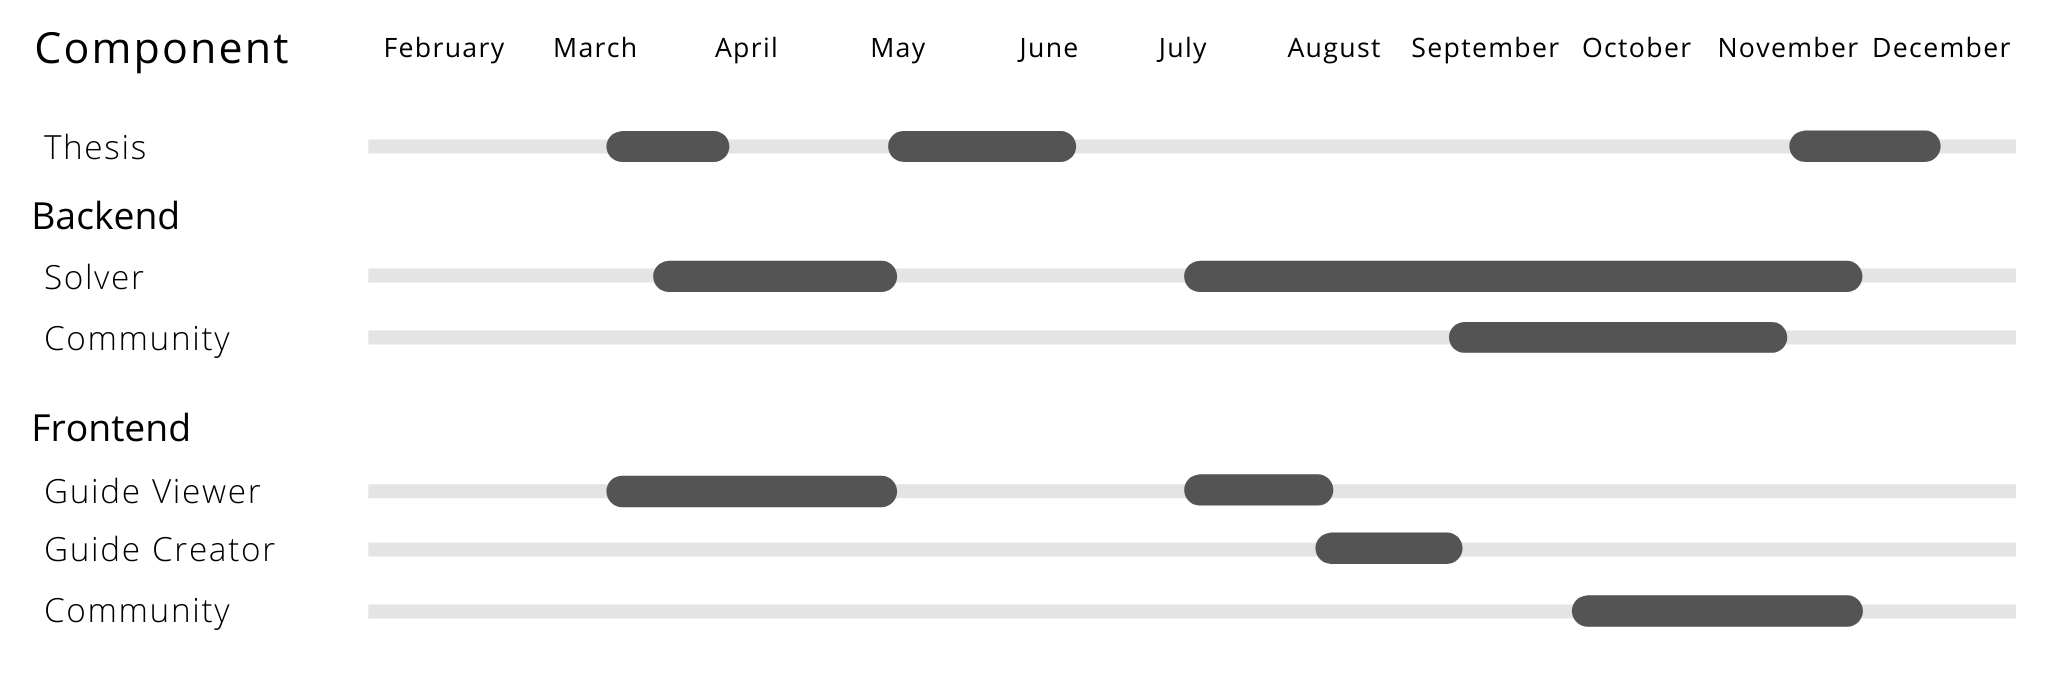
\includegraphics[width=1.01\textwidth]{assets/4-component-timeline.png}
\end{figure}

As can be seen, the work has been pretty well planned and thought out. The actual development time spans the whole project time frame.

The figure below presents the estimated intensity of work.

\begin{figure}[H]
	\label{04-commit-intensity}
	\caption{The project contributions graph - the number of commits to the \texttt{master} branch.}
  \centering
    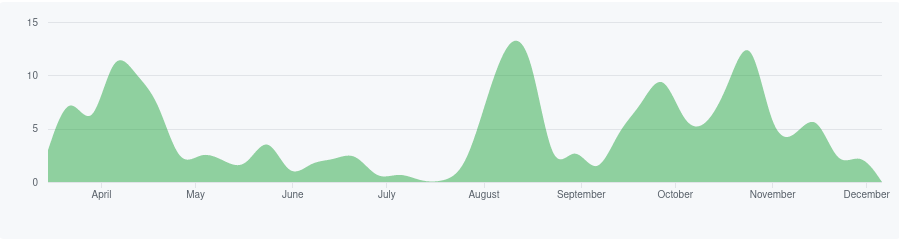
\includegraphics[width=1.01\textwidth]{assets/4-contributions-graph.png}
\end{figure}

The more detailed monthly breakdown of the project state, with features on which we worked, is listed below.

\subsubsection{March}

At the beginning of March we were looking for a supervisor, formulating problems, and planning the project.

\medskip

Having all the formal issues sorted out, we started the Topic Research phase.

Most of the time was spent on studying the \textit{Geometric folding algorithms: Linkages, Origami, Polyhedra} course\cite{mit-course}. The videos provided us with knowledge concerning the scientific field of computational origami, and most importantly:
\begin{itemize}
	\item the terminology,
	\item current numerical algorithms for paper solving problems,
	\item on-going research,
	\item a file format for saving crease patterns,
	\item pitfalls to avoid.
\end{itemize}

It is hard to imagine this project coming to fruition without getting familiar with the aforementioned course.

\subsubsection{April}

April was the start of the Development phase.

We started prototyping, in parallel, the following components:
\begin{itemize}
	\item the Guide Viewer
	\item the Solver.
\end{itemize}

Most notable features that were completed in April include:
\begin{itemize}
	\item adapting the \tech{.fold} file specification to suit the project needs,
	\item \tech{.fold} file parsing on both the backend and the frontend,
	\item \tech{.fold} file rendering on the frontend,
	\item the frontend deployment pipeline,
	\item triangulation on the backend.
\end{itemize}
The end of April resulted in first prototypes being previewed and discussed. Our vision of the project was materializing.

\begin{figure}[H]
	\label{04-first-prototypes}
	\caption{The Guide Viewer at the end of April}
  \centering
    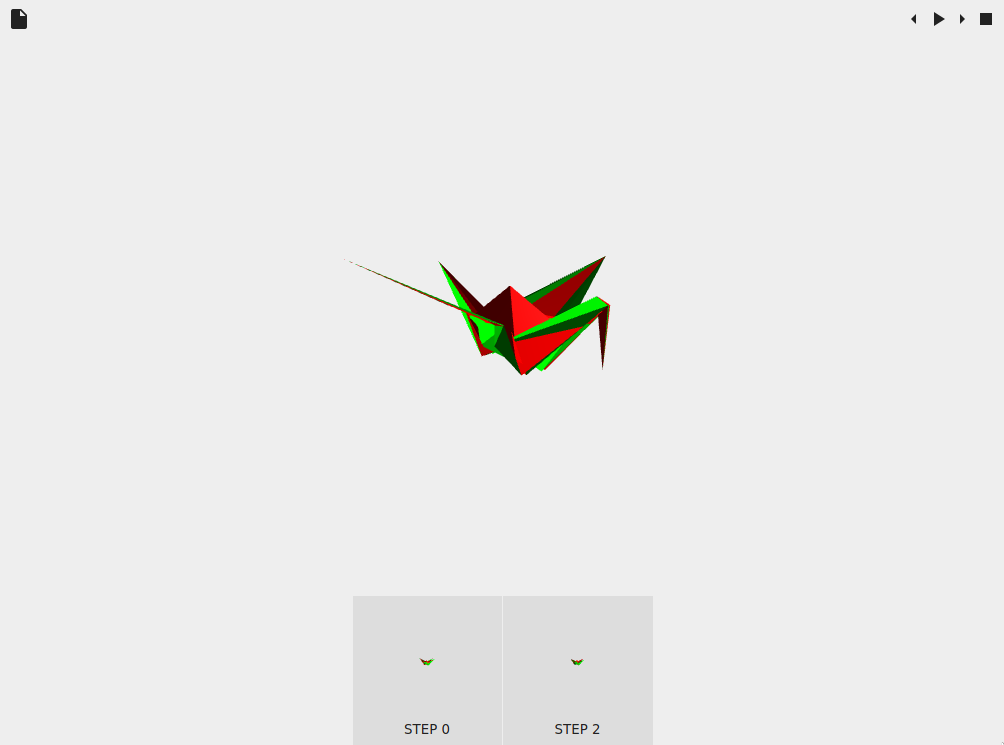
\includegraphics[width=1.01\textwidth]{assets/prototype-front.png}
\end{figure}


% 05-11.04 - FOLD preview prototype
% 12-18.04 - Rewrite in react, file loader, code quality enforcement
% 19-25.04 - Continuous integration setup, lightning changes, solver 
% 24.05-30.05 - Thesis, solver

\subsubsection{May}

During May we refactored the prototype that was developed in April. We adjusted our technology choices and introduced testing libraries.

The most notable aspects that were completed in May include:

\begin{itemize}
	\item first working prototype of the Solver
	\item incorporation of the React framework into the frontend,
	\item the first chapter of the thesis. 
\end{itemize}

\subsubsection{June}

The main topic for May and June was the second chapter of the thesis. The prototype section was written during that time.

\subsubsection{July}

July was not a fruitful month for the project. Several discussions were held, but no actual progress was made.

\subsubsection{August}

In August our focus shifted to performance and stability aspects of the system. 

The most important matters that were wrapped up in August consist of:

\begin{itemize}
	\item adding a damping force to the Solver,
	\item switching the Solver's runtime environment to PyPy,
	\item adding Continuous Integration to the Solver,
	\item supporting target angles in the Solver,
	\item displaying edges with their assignment on the model,
	\item adding timeline scrubbing to the Guide Viewer.
\end{itemize}

\subsubsection{September}

September was a productive time, which brought a lot of business value to the application. 

This time we undertook the implementation of Guide Creator and Community backend parts of the system.
\medskip
We accomplished:

\begin{itemize}
	\item smooth animations with an addition of Guide encoding,
	\item a possibility to compose and create Guides intuitively using the Guide Creator,
\end{itemize}

\subsubsection{October}

In October, we continued working on the community aspect of the system. 

The most valuable features completed in October include:

\begin{itemize}
	\item option to create an account,
	\item ability to log in,
	\item Guide upload functionality,
	\item password reset form,
	\item ability to like a Guide,
	\item Guides Browser,
	\item support for 2D crease patterns.
\end{itemize}


\subsubsection{November}
% 01.11-07.11 - Multi-crease select, triangulation changes, color tweaking,
% 08.11-14.11 - Updating, deleting guides
% 15.11-21.11 - Community backend deployment
% 22.11-now - Thesis, bugfixing

At the beginning of November, we had an application with almost all functional requirements covered. It needed some tweaking, mainly from the User Experience and User Interface points of view. The deadline was nigh. Therefore, we focused all our attention on wrapping up the development process and gaining momentum on writing the paper.

\medskip

We have:

\begin{itemize}
	\item eliminated most of the major pain points from the system,
	\item added Guide deleting and updating functionalities,
	\item widened crease pattern support by changing the triangulation algorithm,
	\item improved visual aspects of the system.
\end{itemize}


\subsubsection{December}

As stated previously, in December we buckled down to writing the thesis and fulfilling formal requirements.

\clearpage

\section{\SectionTitleResults}
\label{sec:wyniki-projektu}
\subsection{Summary of product functionality}
% Podsumowanie (przegląd) zrealizowanych funkcji finalnego produktu
% Ilustracje (screenshoty) do omawianych funkcji. Mile widziane są opis poszczególnych okien ze wskazaniem co na nich widać

In the \nameref{section:functional-requirements} section we have defined Folder's and Designer's user stories and assigned priorities to them.
All the requirements of priority 3 (high) have been realized.
Almost all the requirements of priority 2 (medium) have been resolved.
And most of the requirements of priority 1 (low) have been addressed as well.
\smallskip

In this section we have reviewed the covered functionality from the end user's perspective using screenshots of the end product.
Each section presents some part of the application and lists user stories that are addressed in a given view.
Overlaid on the screenshots are markers that describe which functionality is addressed in which part of the UI.
The format of each marker is $NX$, where $N$ is a letter - either $F$ or $D$ depicting whether  
the highlighted part of the UI corresponds to a \textbf{F}older's user story or a \textbf{D}esigner's user story.
And $X$ represents a user story's sequence number, assigned to it previously in the section \nameref{section:functional-requirements}.

\subsubsection{Guide Viewer}

Folder's user stories:
\begin{enumerate}
	\setcounter{enumi}{0}
	\requirement{3}{load an Instruction}
	\requirement{3}{view the 3D representation of the Instruction step}
	\requirement{3}{switch to the next step in the Instruction}
	\requirement{3}{switch to the previous step in the Instruction}
	\requirement{3}{see the Transition between two Instruction steps}
	\requirement{2}{pause the Transition at any time}
	\requirement{2}{rewind the Transition}
	\requirement{2}{forward the Transition}
	\requirement{3}{rotate the Model in 3D space}
	\requirement{3}{zoom the Model in and out in 3D space}
	\requirement{1}{see creases of the Model} 
	\requirement{2}{distinguish paper's top and bottom sides} 

	\setcounter{enumi}{13}

	\requirement{3}{navigate between simulator and community views} 
\end{enumerate}

\begin{figure}[H]
  	\centering
    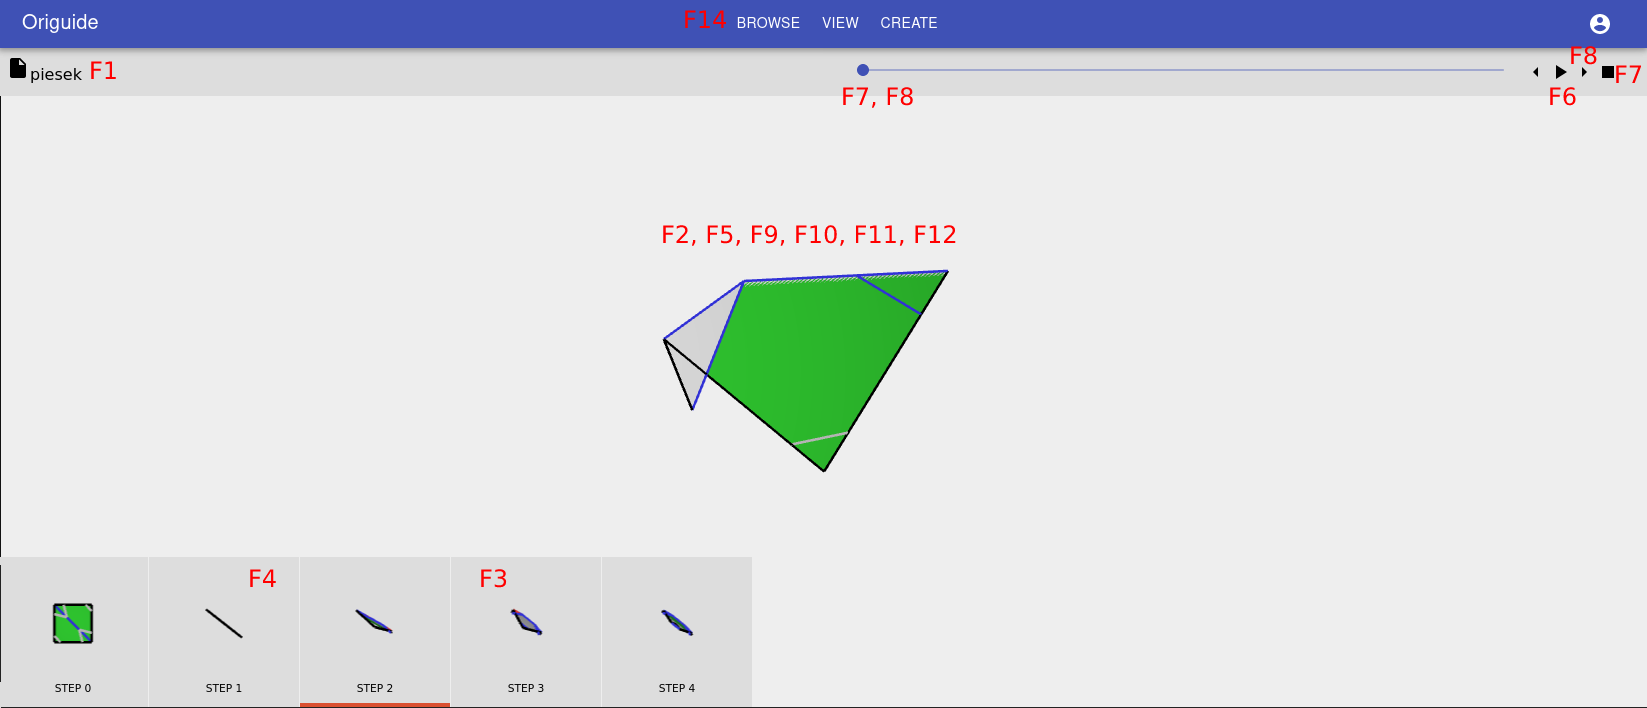
\includegraphics[width=\textwidth]{assets/5-guideViewer.png}
\end{figure}

\subsubsection{Guide Browser}

Folder's user stories:
\begin{enumerate}
	\setcounter{enumi}{14}
	\requirement{3}{view Instructions uploaded by other users} 
\end{enumerate}

Designer's user stories:
\begin{enumerate}
	\setcounter{enumi}{0}
	\requirement{3}{upload an Instruction}
	\requirement{3}{view my Instructions}
	\requirement{3}{delete my Instructions}
	\requirement{3}{update my Instructions}
\end{enumerate}

\begin{figure}[H]
  	\centering
    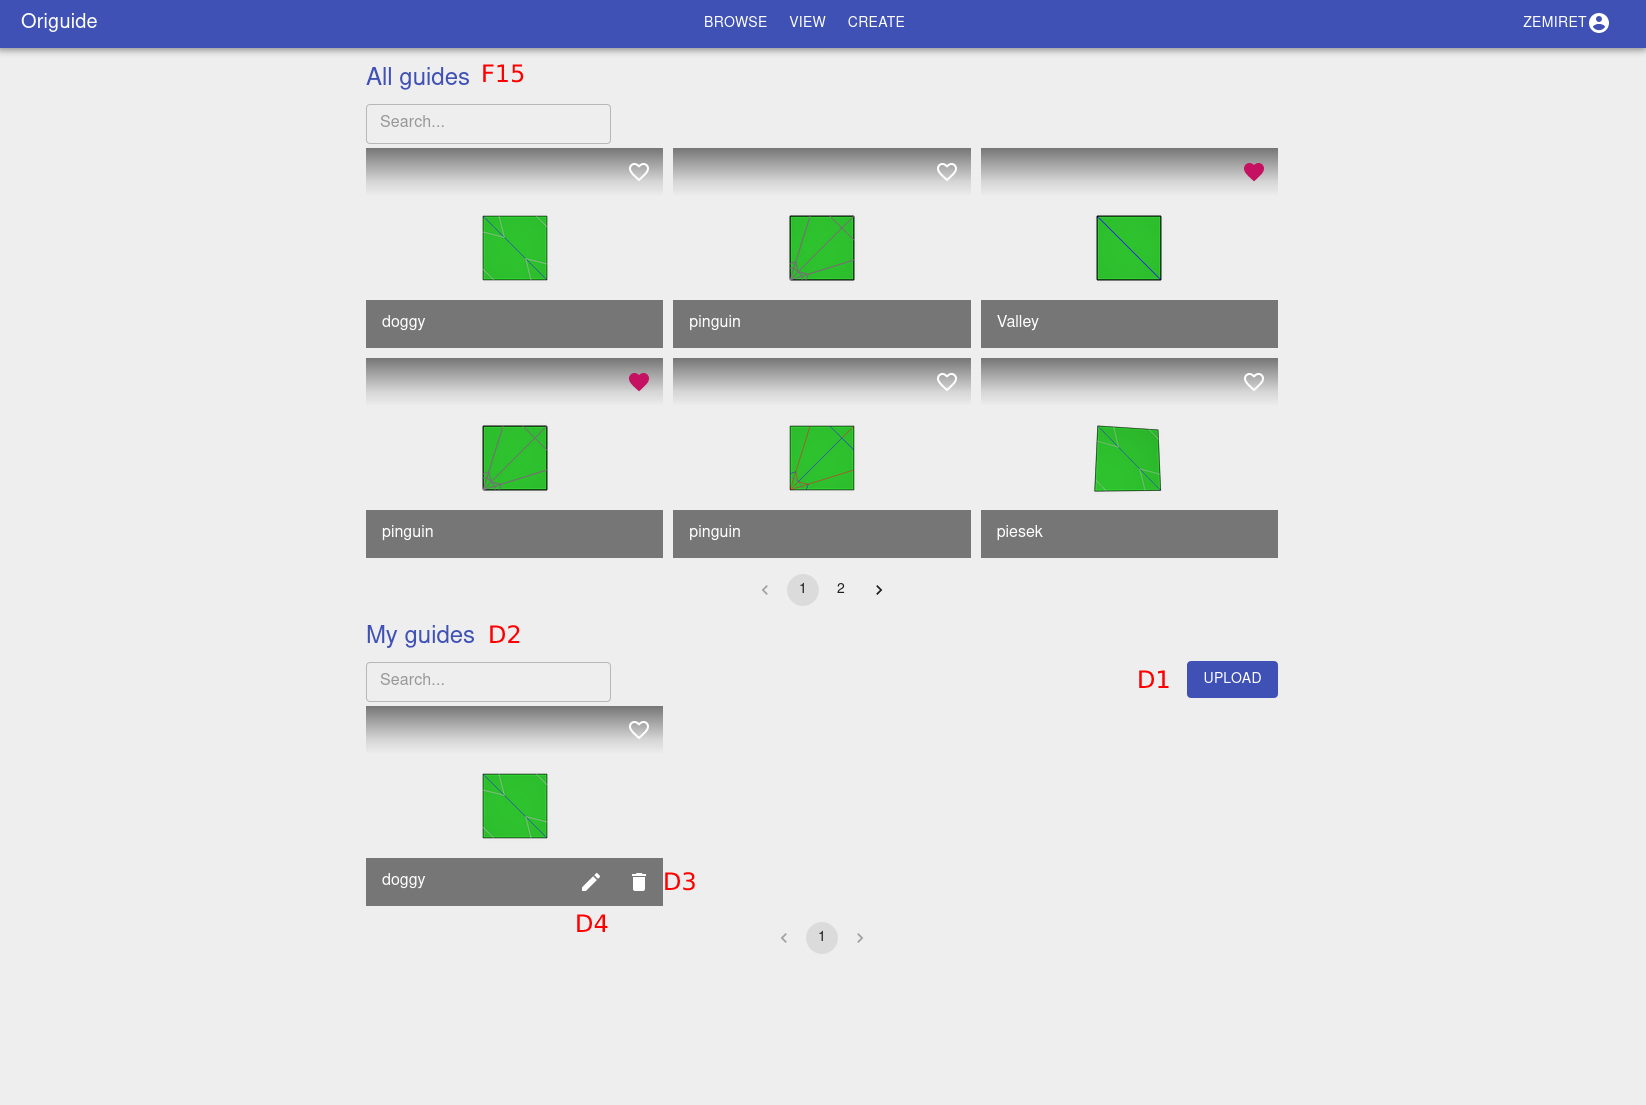
\includegraphics[width=\textwidth]{assets/5-guideBrowser.png}
\end{figure}

\subsubsection{Guide Creator}

Designer's user stories:
\begin{enumerate}
	\setcounter{enumi}{4}
	\requirement{1}{mark my Instructions as public or private}
	\requirement{1}{visually design an Instruction}
	\requirement{1}{save a designed Instruction}
\end{enumerate}

\begin{figure}[H]
  	\centering
    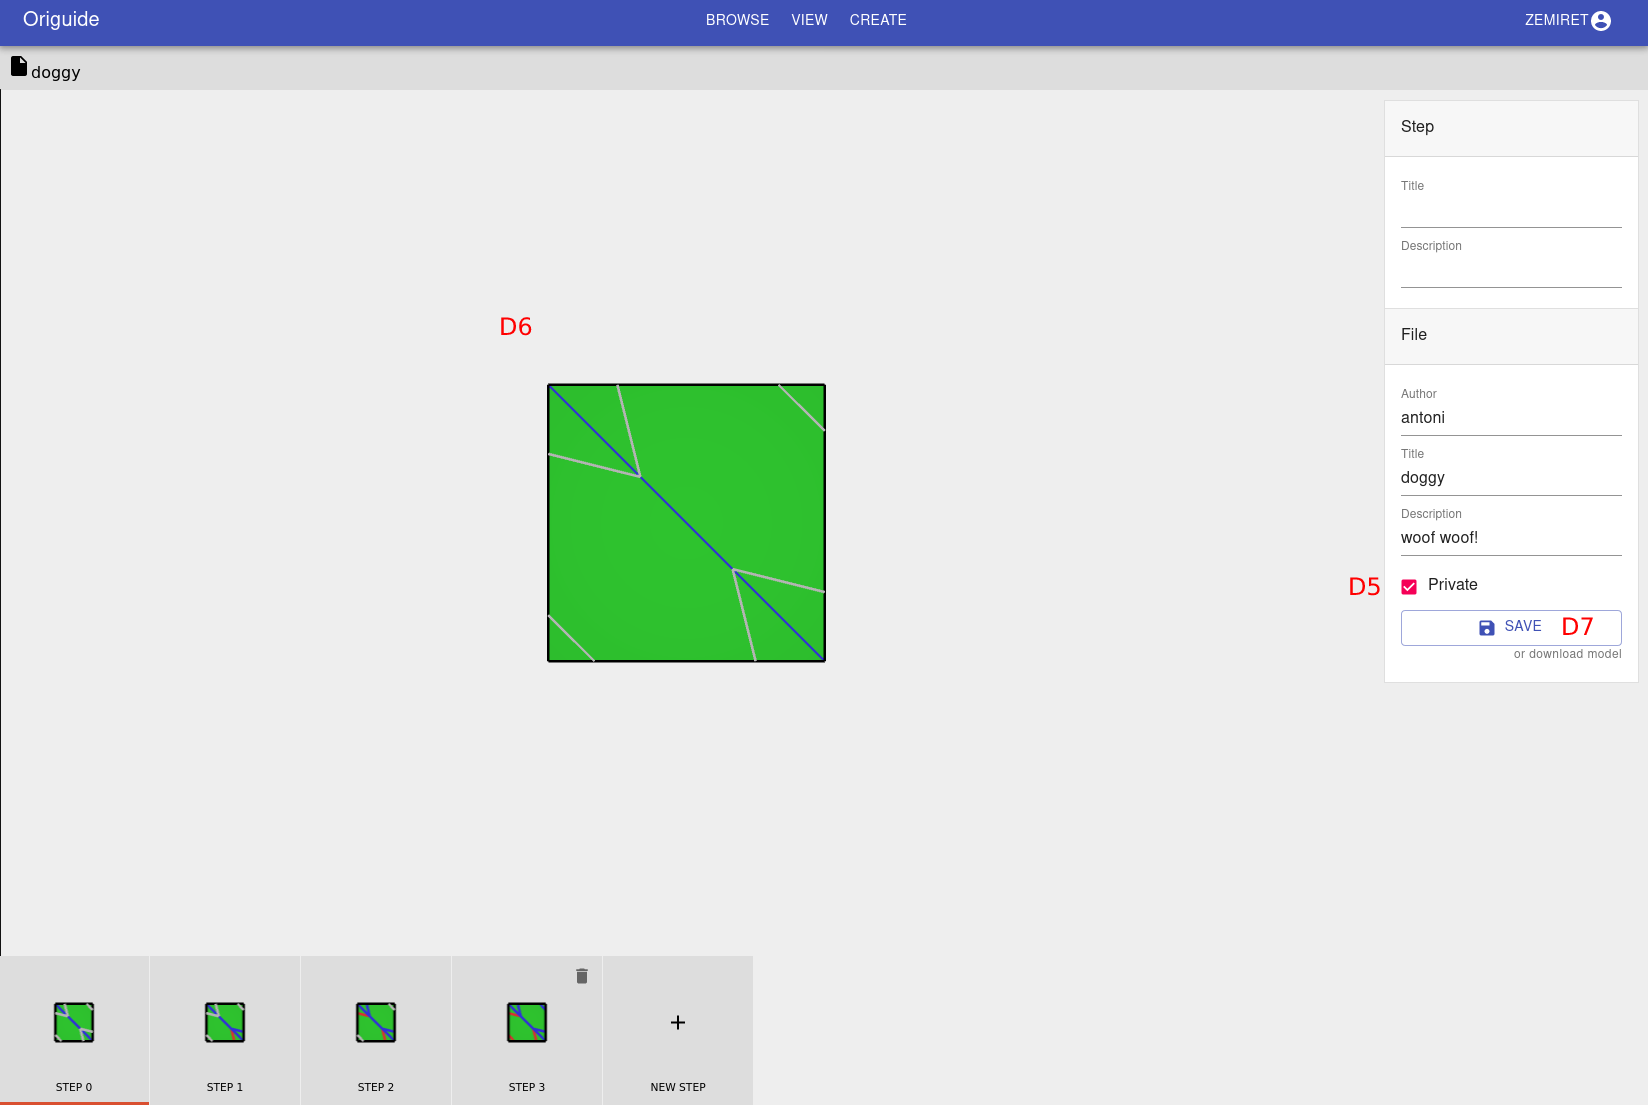
\includegraphics[width=\textwidth]{assets/5-guideCreator.png}
\end{figure}

\subsubsection{Sign up}

Folder's user stories:
\begin{enumerate}
	\setcounter{enumi}{15}
	\requirement{3}{create an account} 
\end{enumerate}

\begin{figure}[H]
  	\centering
    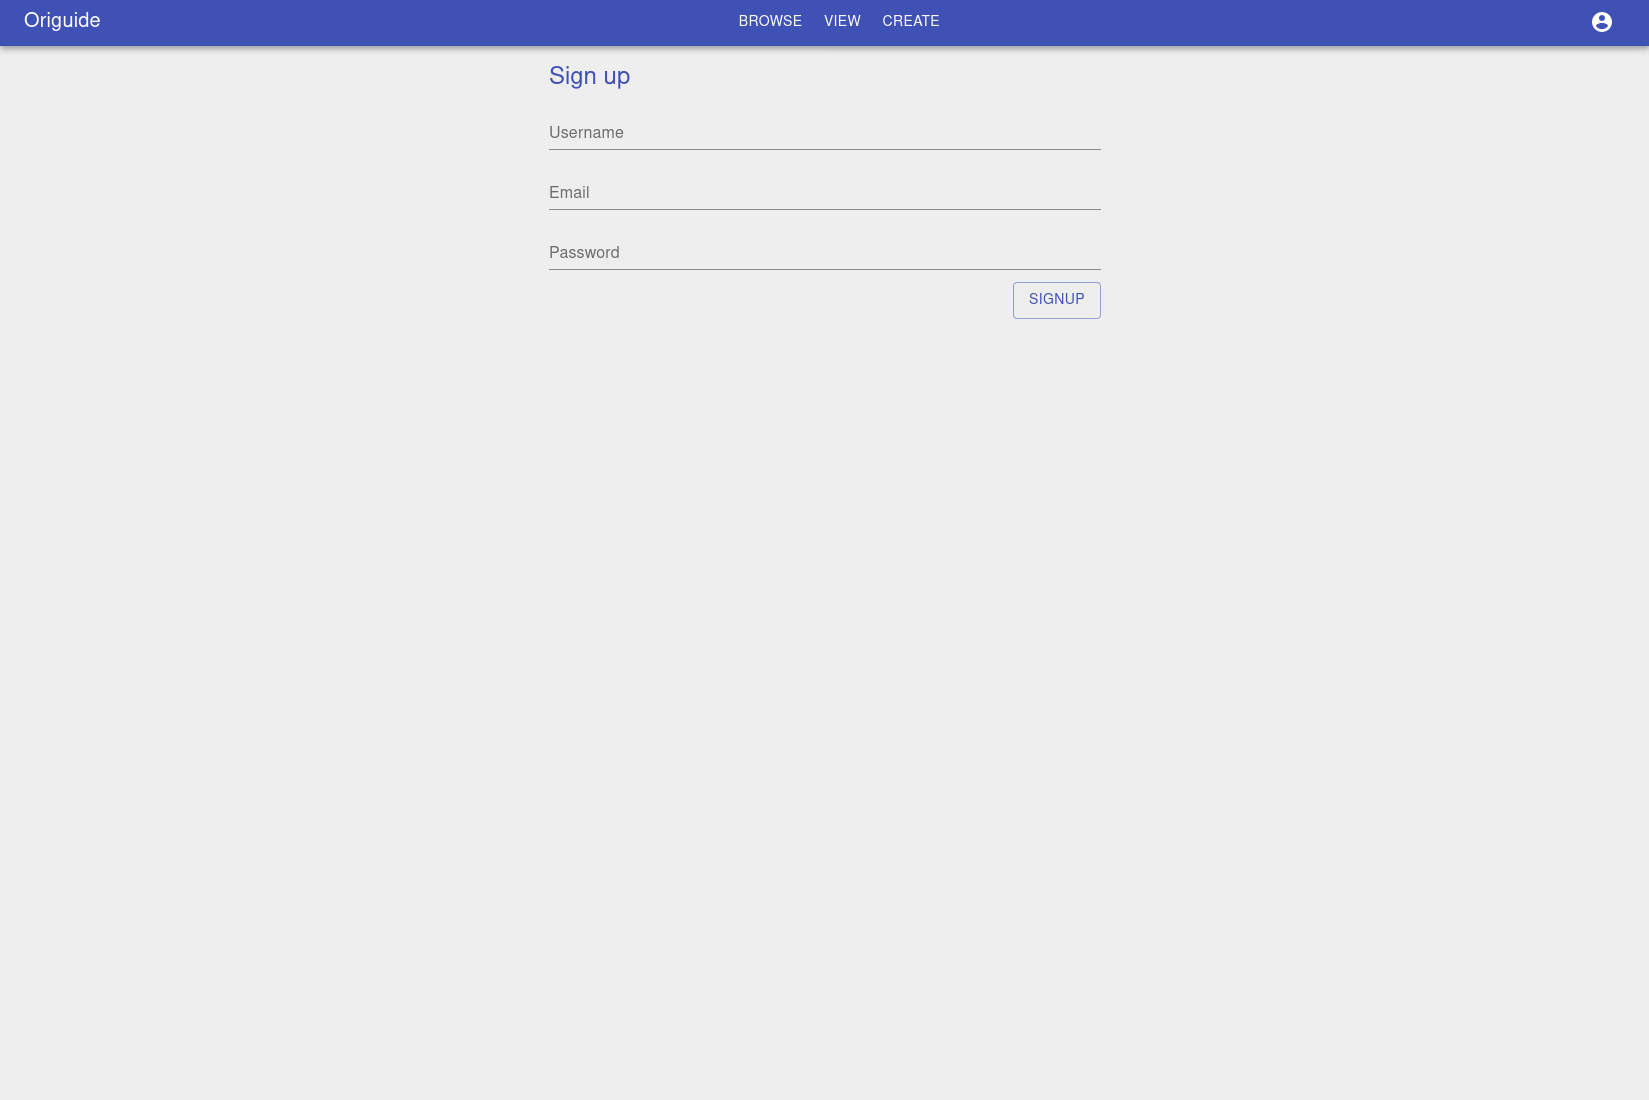
\includegraphics[width=\textwidth]{assets/5-signUp.png}
\end{figure}

\subsubsection{Sign in}

Folder's user stories:
\begin{enumerate}
	\setcounter{enumi}{16}
	\requirement{3}{log into the system} 
\end{enumerate}

\begin{figure}[H]
  	\centering
    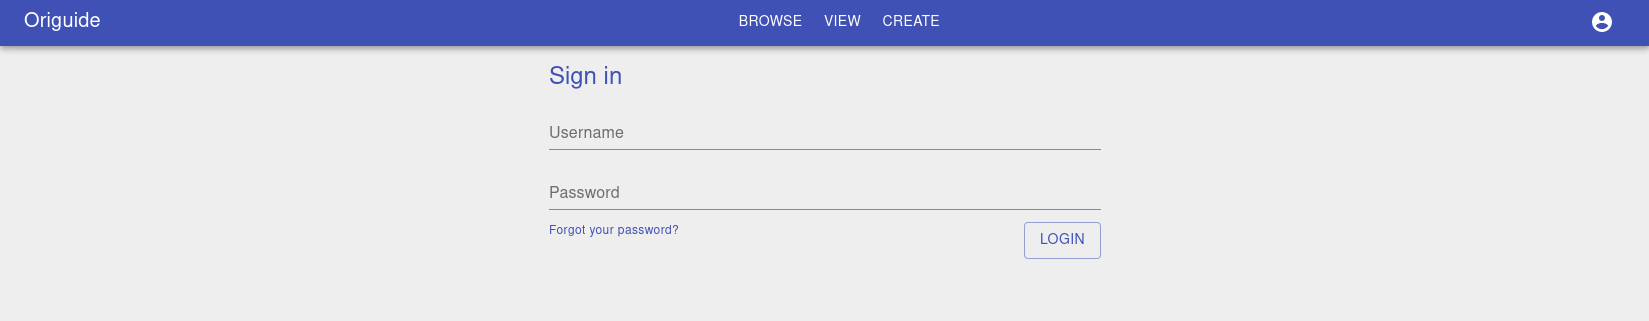
\includegraphics[width=0.95\textwidth]{assets/5-signIn.png}
\end{figure}

\subsubsection{Reset password}

Folder's user stories:
\begin{enumerate}
	\setcounter{enumi}{17}
	\requirement{3}{reset the password} 
\end{enumerate}

\begin{figure}[H]
  	\centering
    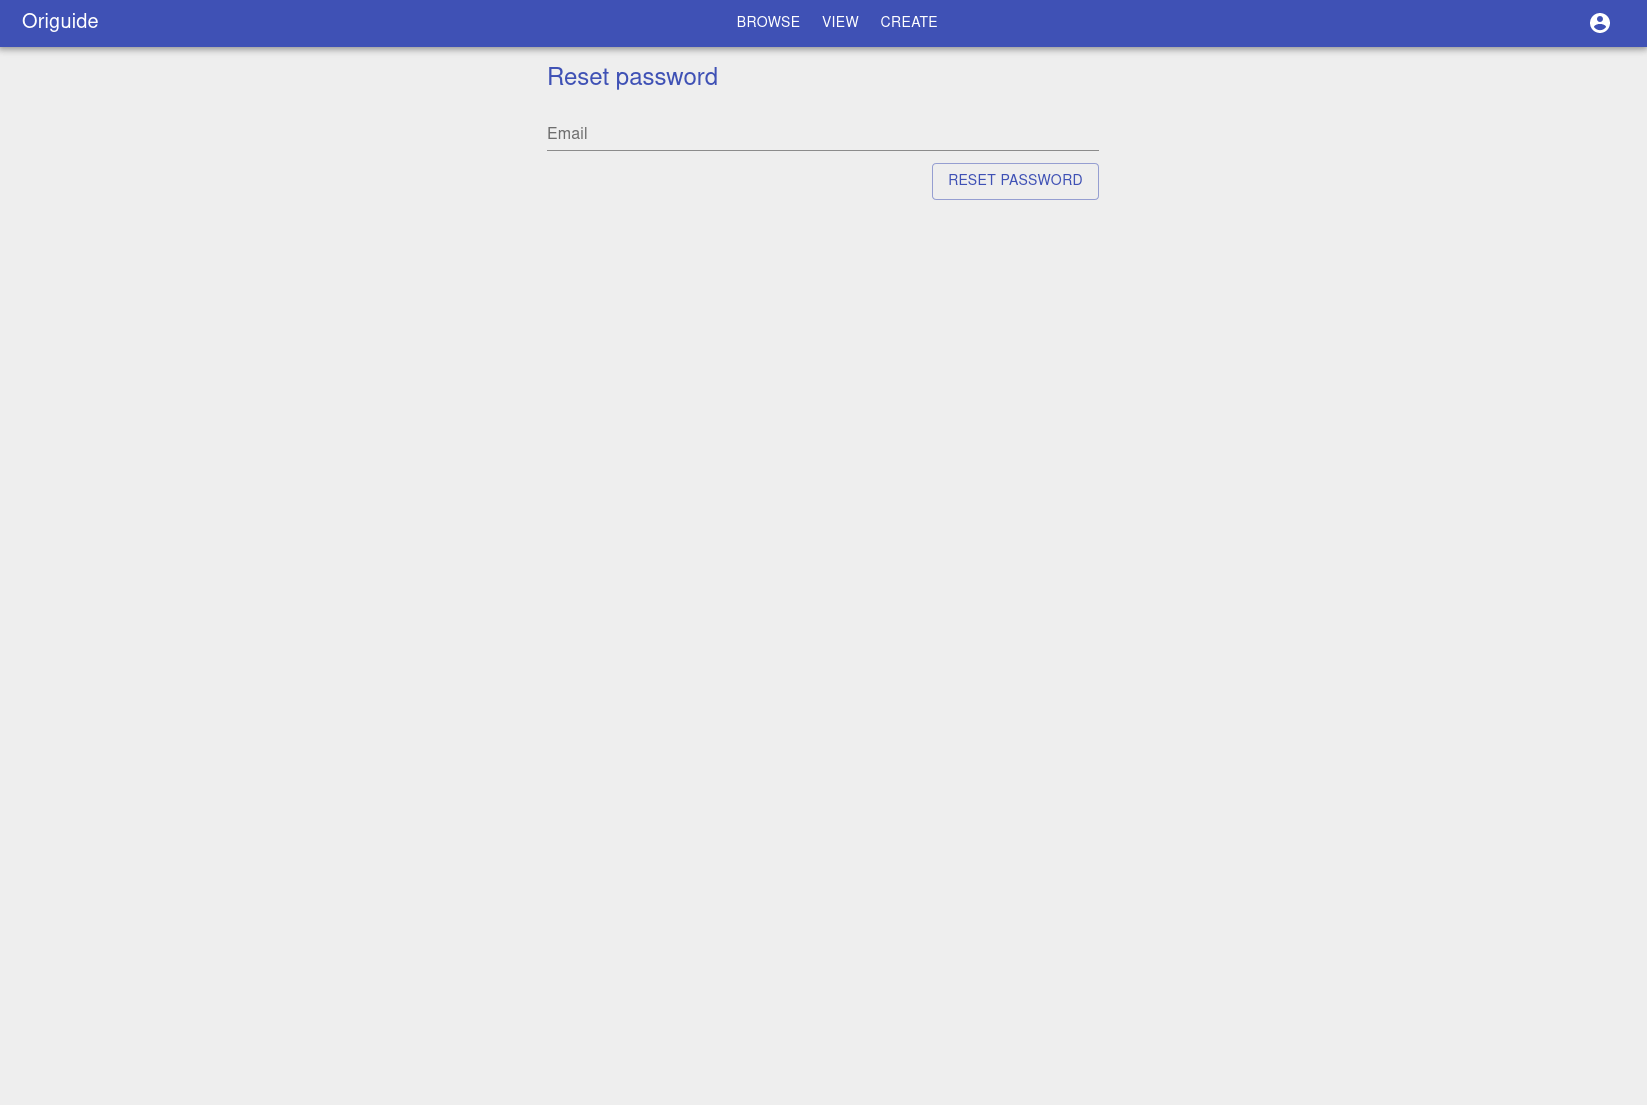
\includegraphics[width=0.95\textwidth]{assets/5-passwordResetForm.png}
\end{figure}

Once the form is submitted, the user receives an email containing password reset instructions.

\begin{figure}[H]
  	\centering
    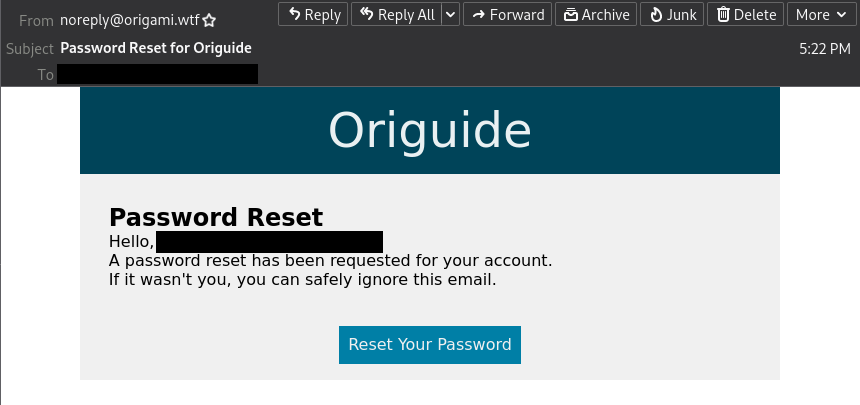
\includegraphics[width=0.7\textwidth]{assets/5-passwordResetEmail.png}
\end{figure}

\subsubsection{Change password}

Folder's user stories:
\begin{enumerate}
	\setcounter{enumi}{18}
	\requirement{2}{change the password} 
\end{enumerate}

\begin{figure}[H]
  	\centering
    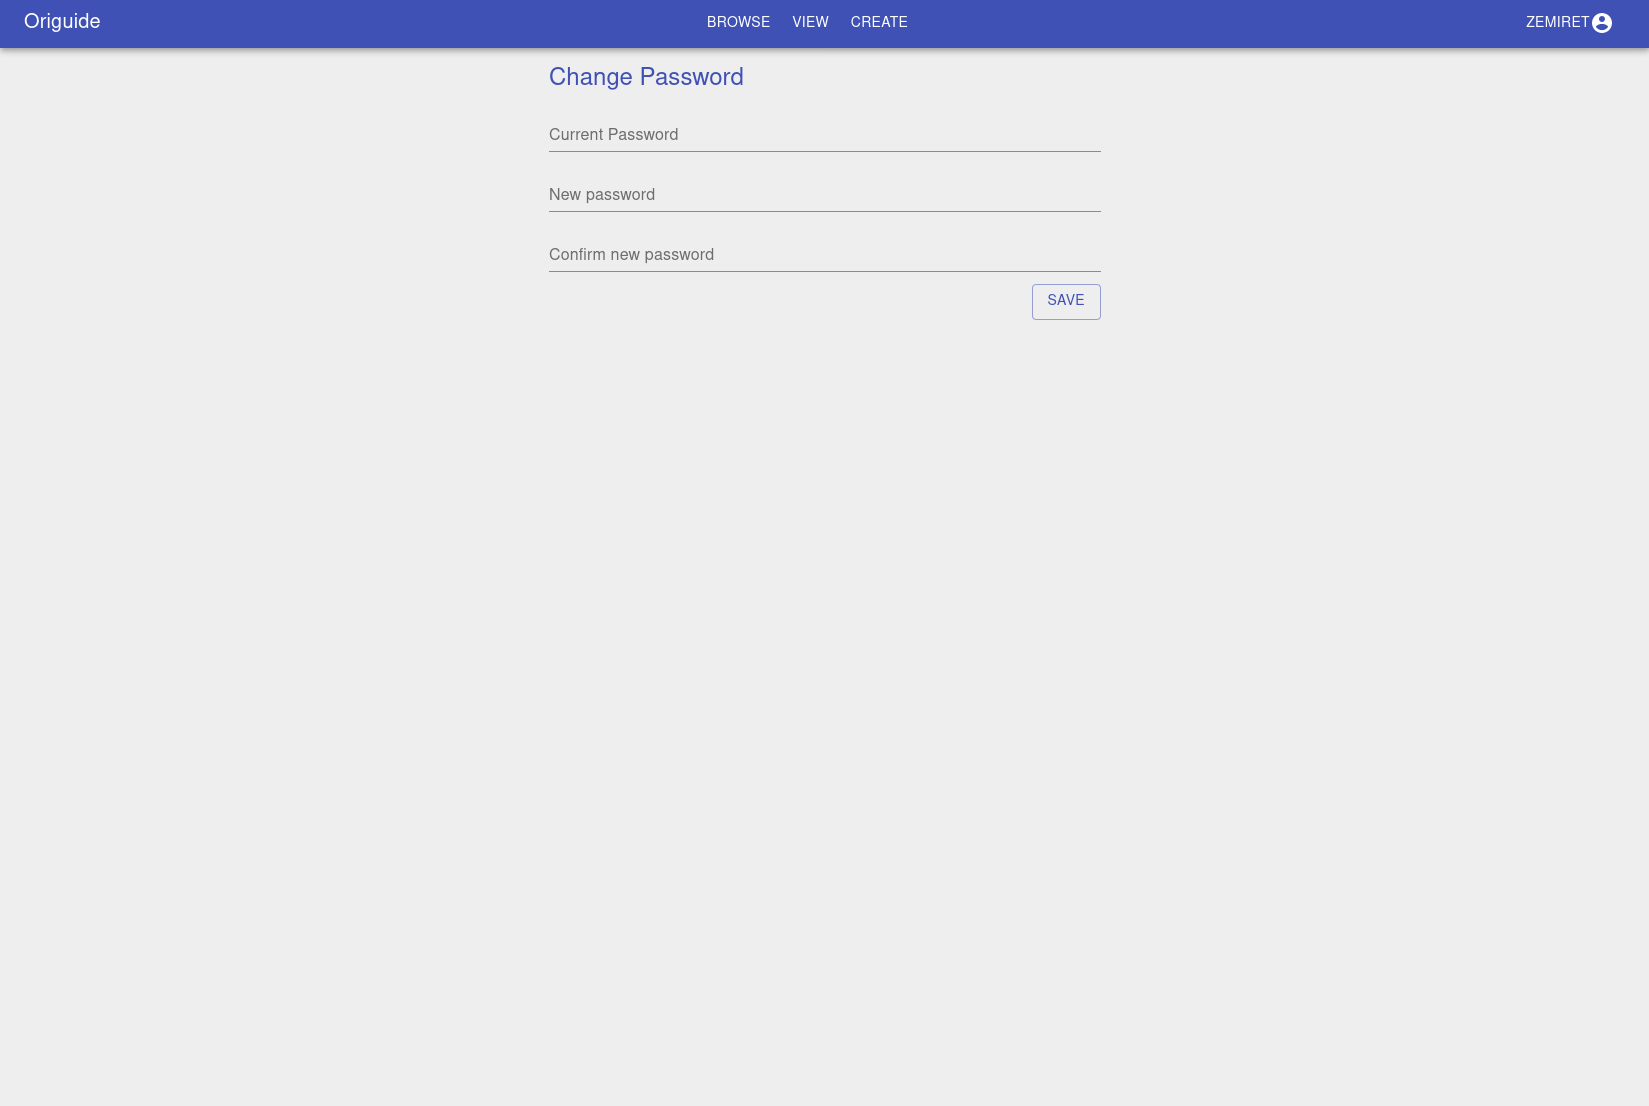
\includegraphics[width=0.95\textwidth]{assets/5-passwordChange.png}
\end{figure}

\subsubsection{Functional requirements that have not been realized}

There are some functional requirements that have not been realized.
All of them happen to be Folder's user stories.
Some proved not to be as important as we had initially assumed.
There are also some that have only been partially accomplished, e.g. they are 
implemented in the backend but no corresponding frontend option is present.
\smallskip

Not realized or partially realized functional requirements:
\begin{enumerate}
	\setcounter{enumi}{12}
	\requirement{1}{change the color of the paper side} 

	
	\setcounter{enumi}{19}
	\requirement{2}{delete the account} 
	\requirement{2}{save another user's Instruction in my account}
	\requirement{1}{mark a saved Instruction as folded} 
\end{enumerate}

\subsubsection{Non-functional requirements}

All but one non-functional requirements have been realized.

The not realized requirement is:
\begin{enumerate}
	\setcounter{enumi}{4}
	\requirement{1}{User should be able to use the application on mobile devices}
\end{enumerate}

Although some parts of our application are usable on mobile devices, 
not everything works as intended. That is not surprising taking into account that
mobile application support had a low priority.

\subsection{Main use cases}
% Prezentacja głównych scenariuszy działania
% Ewentualne skrócone wersje instrukcji (użytkownika, instalacji) - w przypadku kiedy są obszerne proszę je dodać do pracy jako załączniki
% Niekiedy można dodać sekcje FAQ

As defined in the section \nameref{section:project-overview}, there are 2 main 
success paths in the application.
One for Designers and another one for Folders.
These success paths correspond to the main use cases.
In this section we will present these success paths in the context of the end product.

\subsubsection{Designer's success path}

First, the user loads a crease pattern.

\begin{figure}[H]
  	\centering
    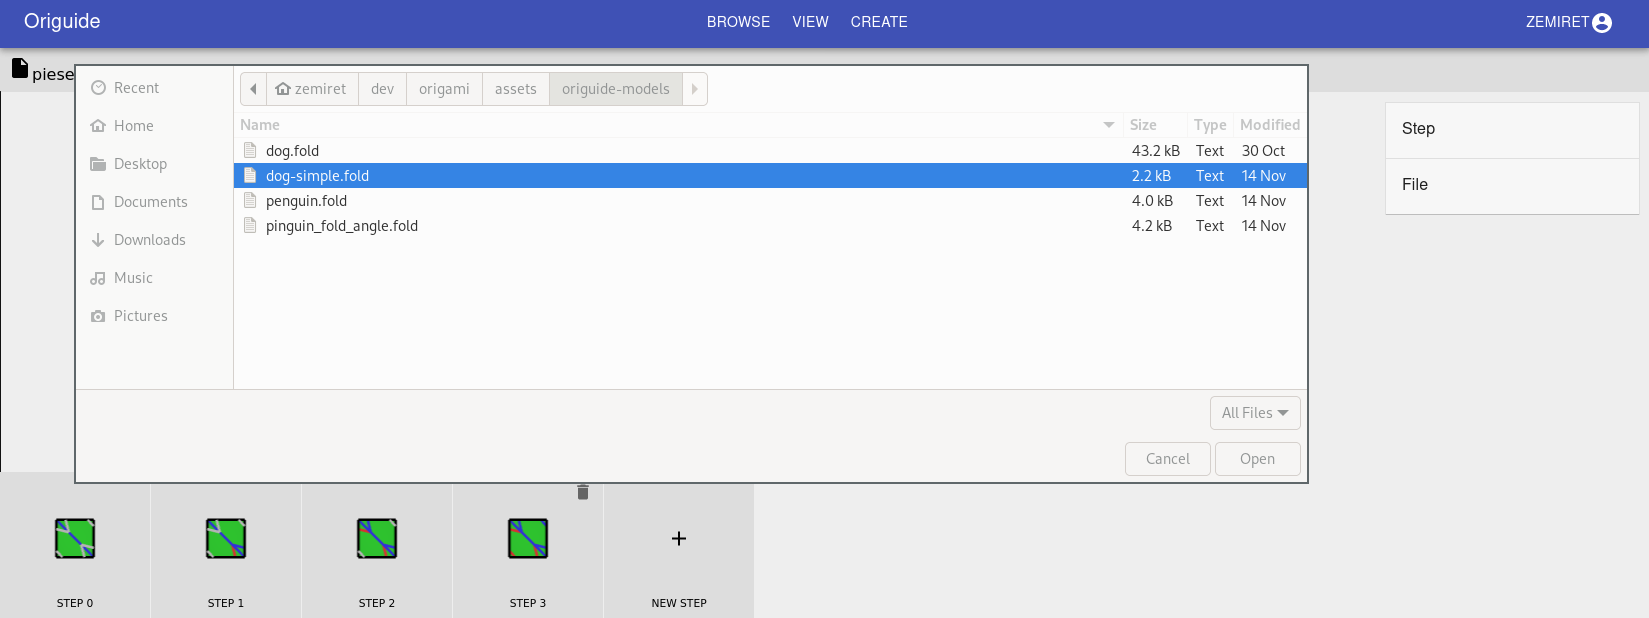
\includegraphics[width=\textwidth]{assets/5-designerLoad.png}
\end{figure}

Next, Guide Creator is shown, and the user proceeds with creating an Instruction.
Once done, the user clicks the \textit{save} button.

\begin{figure}[H]
  	\centering
    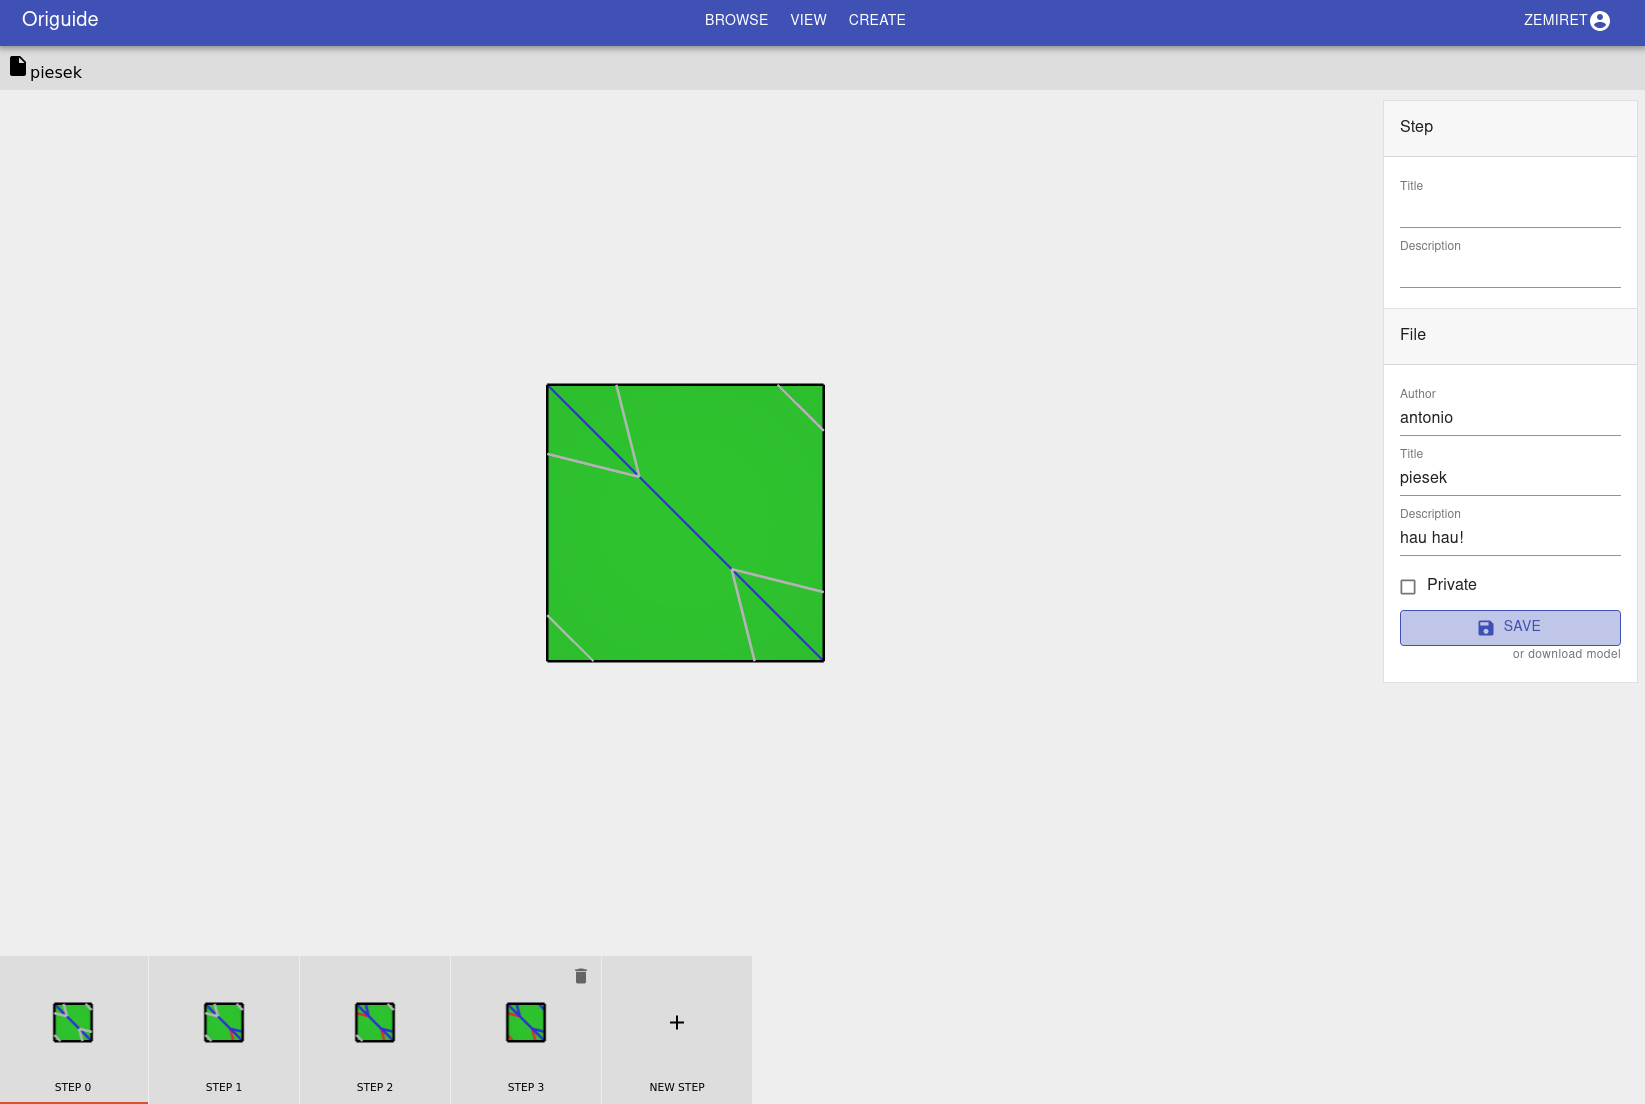
\includegraphics[width=\textwidth]{assets/5-designerSave.png}
\end{figure}

Proper requests are dispatched to the backend, the guide is processed in the background, and
the user is redirected to Guide Browser.

\begin{figure}[H]
  	\centering
    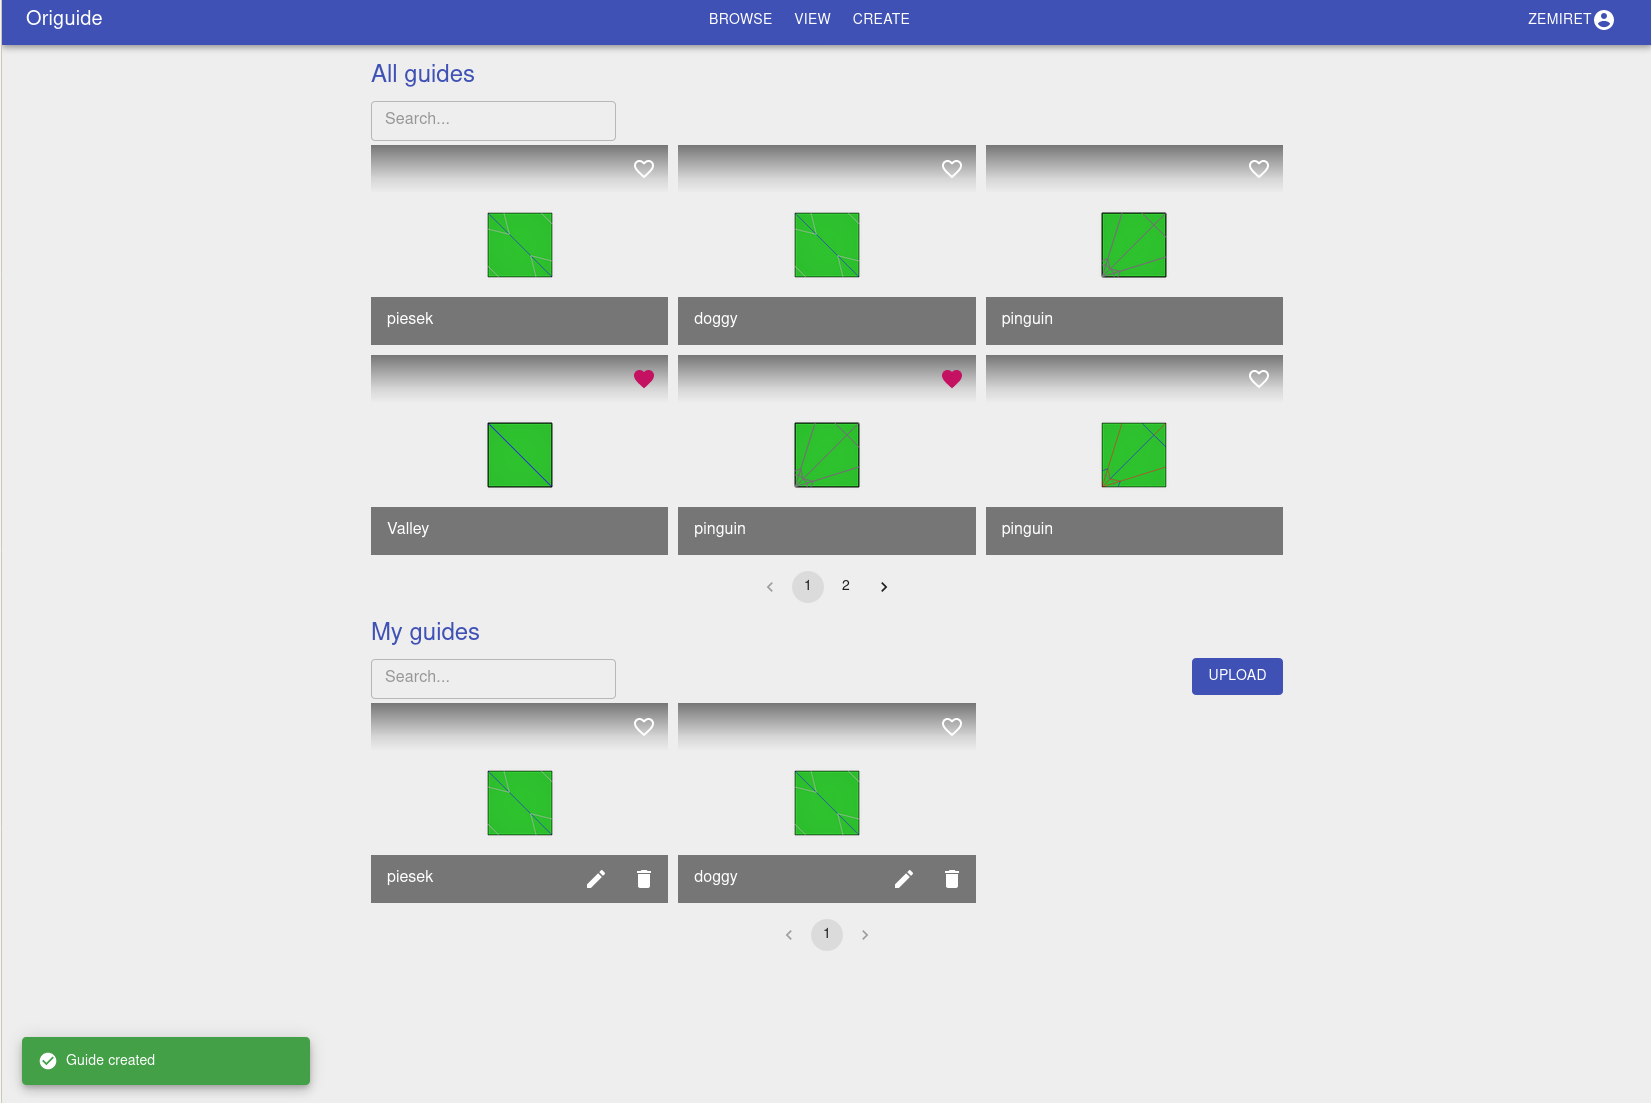
\includegraphics[width=\textwidth]{assets/5-designerBrowser.png}
\end{figure}

\clearpage
\subsubsection{Folder's success path}

The user is presented with Guide Browser. Then, the user clicks on one of the Guides.

\begin{figure}[H]
  	\centering
    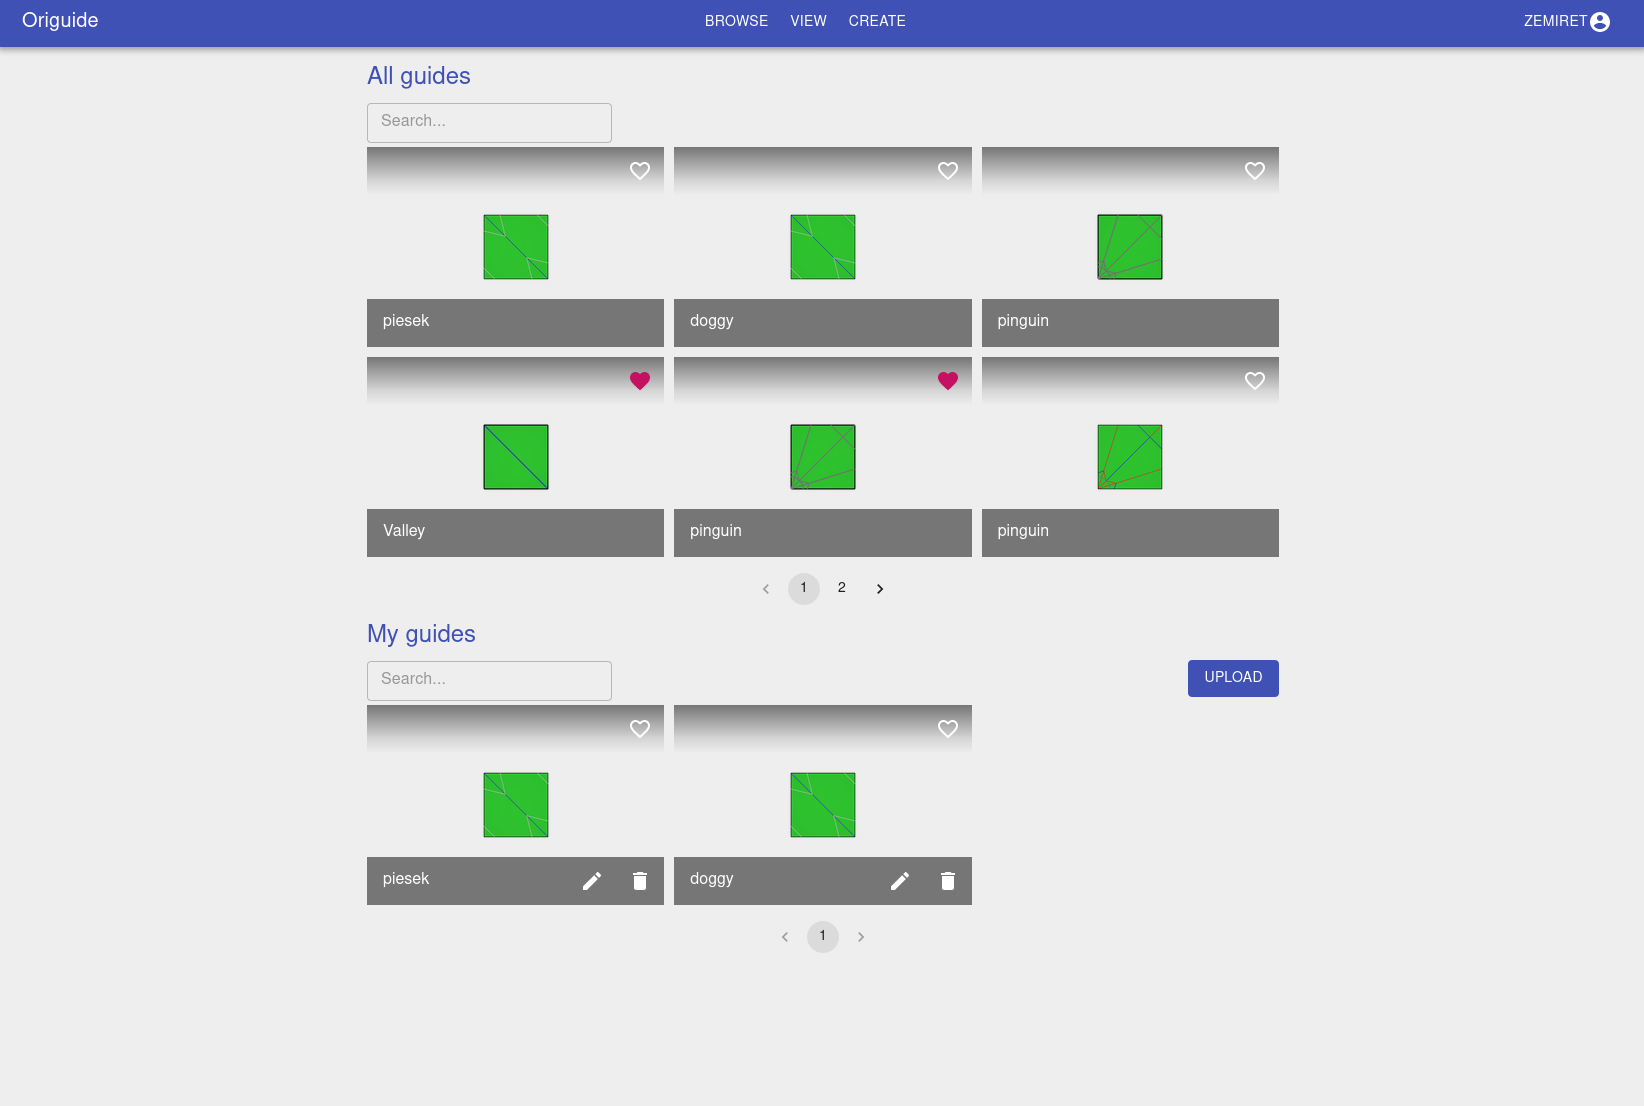
\includegraphics[width=\textwidth]{assets/5-folderOpen.png}
\end{figure}

Once the Guide is loaded, the user is presented with Guide Viewer.

\begin{figure}[H]
  	\centering
    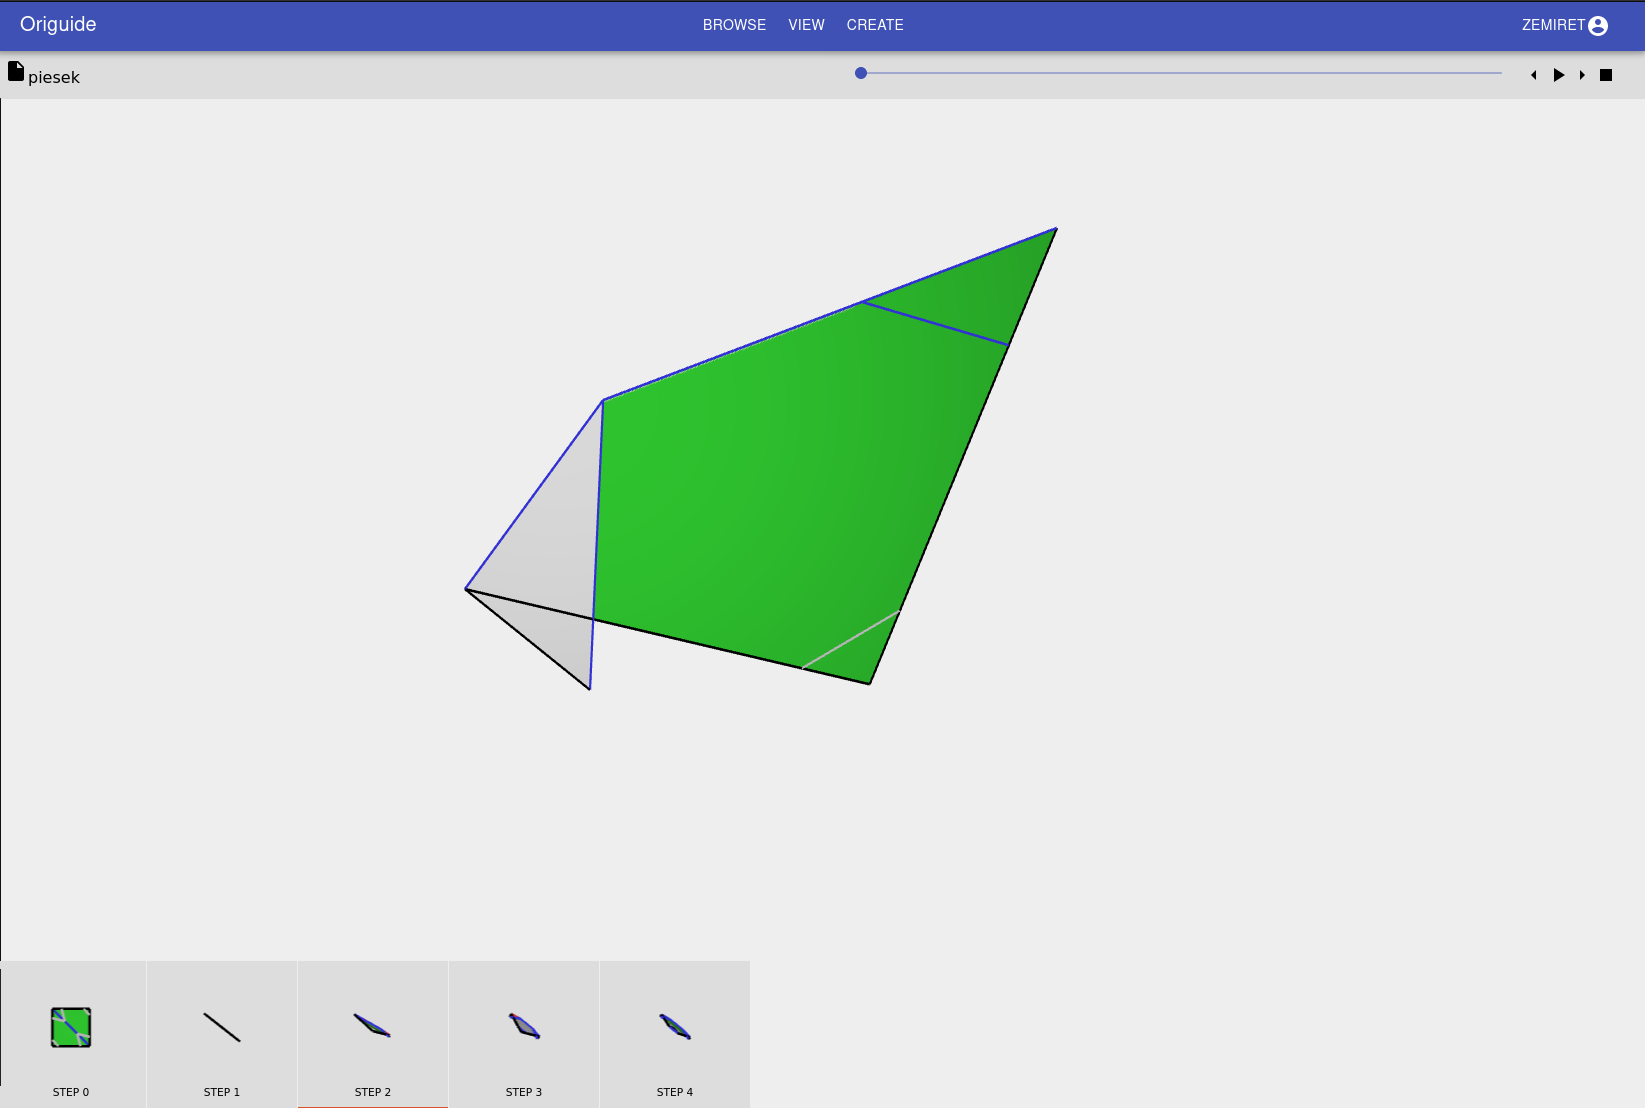
\includegraphics[width=\textwidth]{assets/5-folderView.png}
\end{figure}


\subsection{Project summary}
%Bardzo mile widziane jest podsumowanie wraz z własną subiektywną oceną. Proszę odpowiedzieć sobie i czytelnikowi na pytanie czy projekt się udał, czy jesteście zadowoleni, czy klient jest zadowolony, czego się nauczyliście? Jak można projekt dalej rozwijać?

Overall, we find our project to be a great success.
We have created something interesting both from the scientific and the end user's
point of view. Moreover, our application is something that can be used
by anyone as it is publicly available. Having created the \textit{community}
part of it, we hope to see some real community of origami folders using our product emerge.
\smallskip

Our client seems to be equally happy with the end result.
He appreciates all the work we put into it, 
as well as some more interesting aspects of the project itself.
\smallskip

From the engineering point of view we were confident we can deliver the project.
What at times we found troublesome were some more scientific topics, mostly
connected with how Solver should work.
At some point we were also worried about the performance aspect, but in the end it all worked out well.
During the project we learned a lot about \textit{computational origami} and how to fold a figure or two.
When it comes to the engineering, we did not learn much, but
that is to be expected since we already had some solid foundation in this area.
\smallskip

Although we deem our project complete, it could be developed further as there are a lot of potential areas to work on.
Some of them are:

\begin{itemize}
	\item Collision prevention - although collision detection has been implemented, no prevention is carried out at the moment. At times, this results in some peculiarities during folding.
	\item More sophisticated folding patterns support - right now only figures made out of rigid polygons are supported. In the future, we would like to support some more sophisticated folding patters like inflating or curving.
	\item Improved Guide encoder - folding steps that are produced by Solver are downsampled and encoded to animation frames using some fixed cut-off values. A more robust approach could result in smoother animations.
	\item UI and UX improvements.
	\item Model preview in Guide Creator.
	\item Better thumbnail generation.
\end{itemize}

Even though there is always something more to work on,
both we and our client assumed the current state of the product to be
satisfactory and we are content with the end result.


\clearpage


\bibliography{bibliography}

\end{document}
